\documentclass{article}
\usepackage{float}
\usepackage{fancyhdr}
\usepackage{geometry}
\usepackage{amsmath}
\usepackage{amssymb}
\usepackage{bbm}
\usepackage{listings}
\usepackage{xcolor}
\usepackage{tikz}
\usepackage{hyperref}
\usepackage[parfill]{parskip}

\definecolor{codegreen}{rgb}{0,0.6,0}
\definecolor{codegray}{rgb}{0.5,0.5,0.5}
\definecolor{codepurple}{rgb}{0.58,0,0.82}
\definecolor{backcolour}{rgb}{1,1,1}
 
\lstdefinestyle{mystyle}{
    backgroundcolor=\color{backcolour},   
    commentstyle=\color{codegreen},
    keywordstyle=\color{magenta},
    numberstyle=\tiny\color{codegray},
    stringstyle=\color{codepurple},
    basicstyle=\ttfamily\footnotesize,
    breakatwhitespace=false,         
    breaklines=true,                 
    captionpos=b,                    
    keepspaces=true,                 
    numbers=left,                    
    numbersep=5pt,                  
    showspaces=false,                
    showstringspaces=false,
    showtabs=false,                  
    tabsize=2
}
 
\lstset{style=mystyle}

\parskip = \baselineskip

\pagestyle{fancy}
\lhead{IE 420 Project  \ \ \ \ \ Name: Karl Oskar Julius Olson}
\renewcommand{\headrulewidth}{0.4pt}
\renewcommand{\footrulewidth}{0.4pt}

\title{IE 420 Final Project}
\author{Julius Olson}
\date{April 2020}
\begin{document}

\maketitle{}
\thispagestyle{fancy}

\section*{Question 1}

The implementation was done in \lstinline{C++} to ensure efficient calculations. To make the program more easily readable and to reduce sources of error, the function signature presented in the assignment was altered to \lstinline{binomial(option &opt)}, i.e. a reference to an option struct is sent to the function. The option struct contains (see Appendix \ref{options}) all parameters needed by the CRR binomial function.

\section*{Question 2}
\begin{align*}
	&T=1, K=100, \ S_0 = 100, \ r=0.05, \ q=0.04, \ \sigma = 0.2 \\
	&d_1 = \frac{\ln (S_0 / K) + (r - q + \frac{1}{2}\sigma^2)T}{\sigma \sqrt{T}} \\
	&d_2 = d_1 - \sigma \sqrt{T} \\
	&c_{BS} = S_0e^{-qT}\mathcal{N}_{cdf}(d_1) - Ke^{-rT}\mathcal{N}_{cdf}(d_2)\\
\end{align*}
The price was calculated using the CRR binomial model with the number of steps $N$ increasing until the difference between the CRR price and the Black \& Scholes price was less then $10^{-3}$. Figure \ref{convergence} depicts how the model converges towards the value obtained using the Black-Scholes formula as the value of $N$ is sufficiently large. At $N=1885$ the difference was within the required accuracy and the prices were calculated as:
$$c_{BS} = \$8.102643534, \ c_{CRR} = \$8.103643071$$. The execution time was found to be of magnitude $\mathcal{O}(N^2)$. 
\begin{figure}[H]
	\centering
	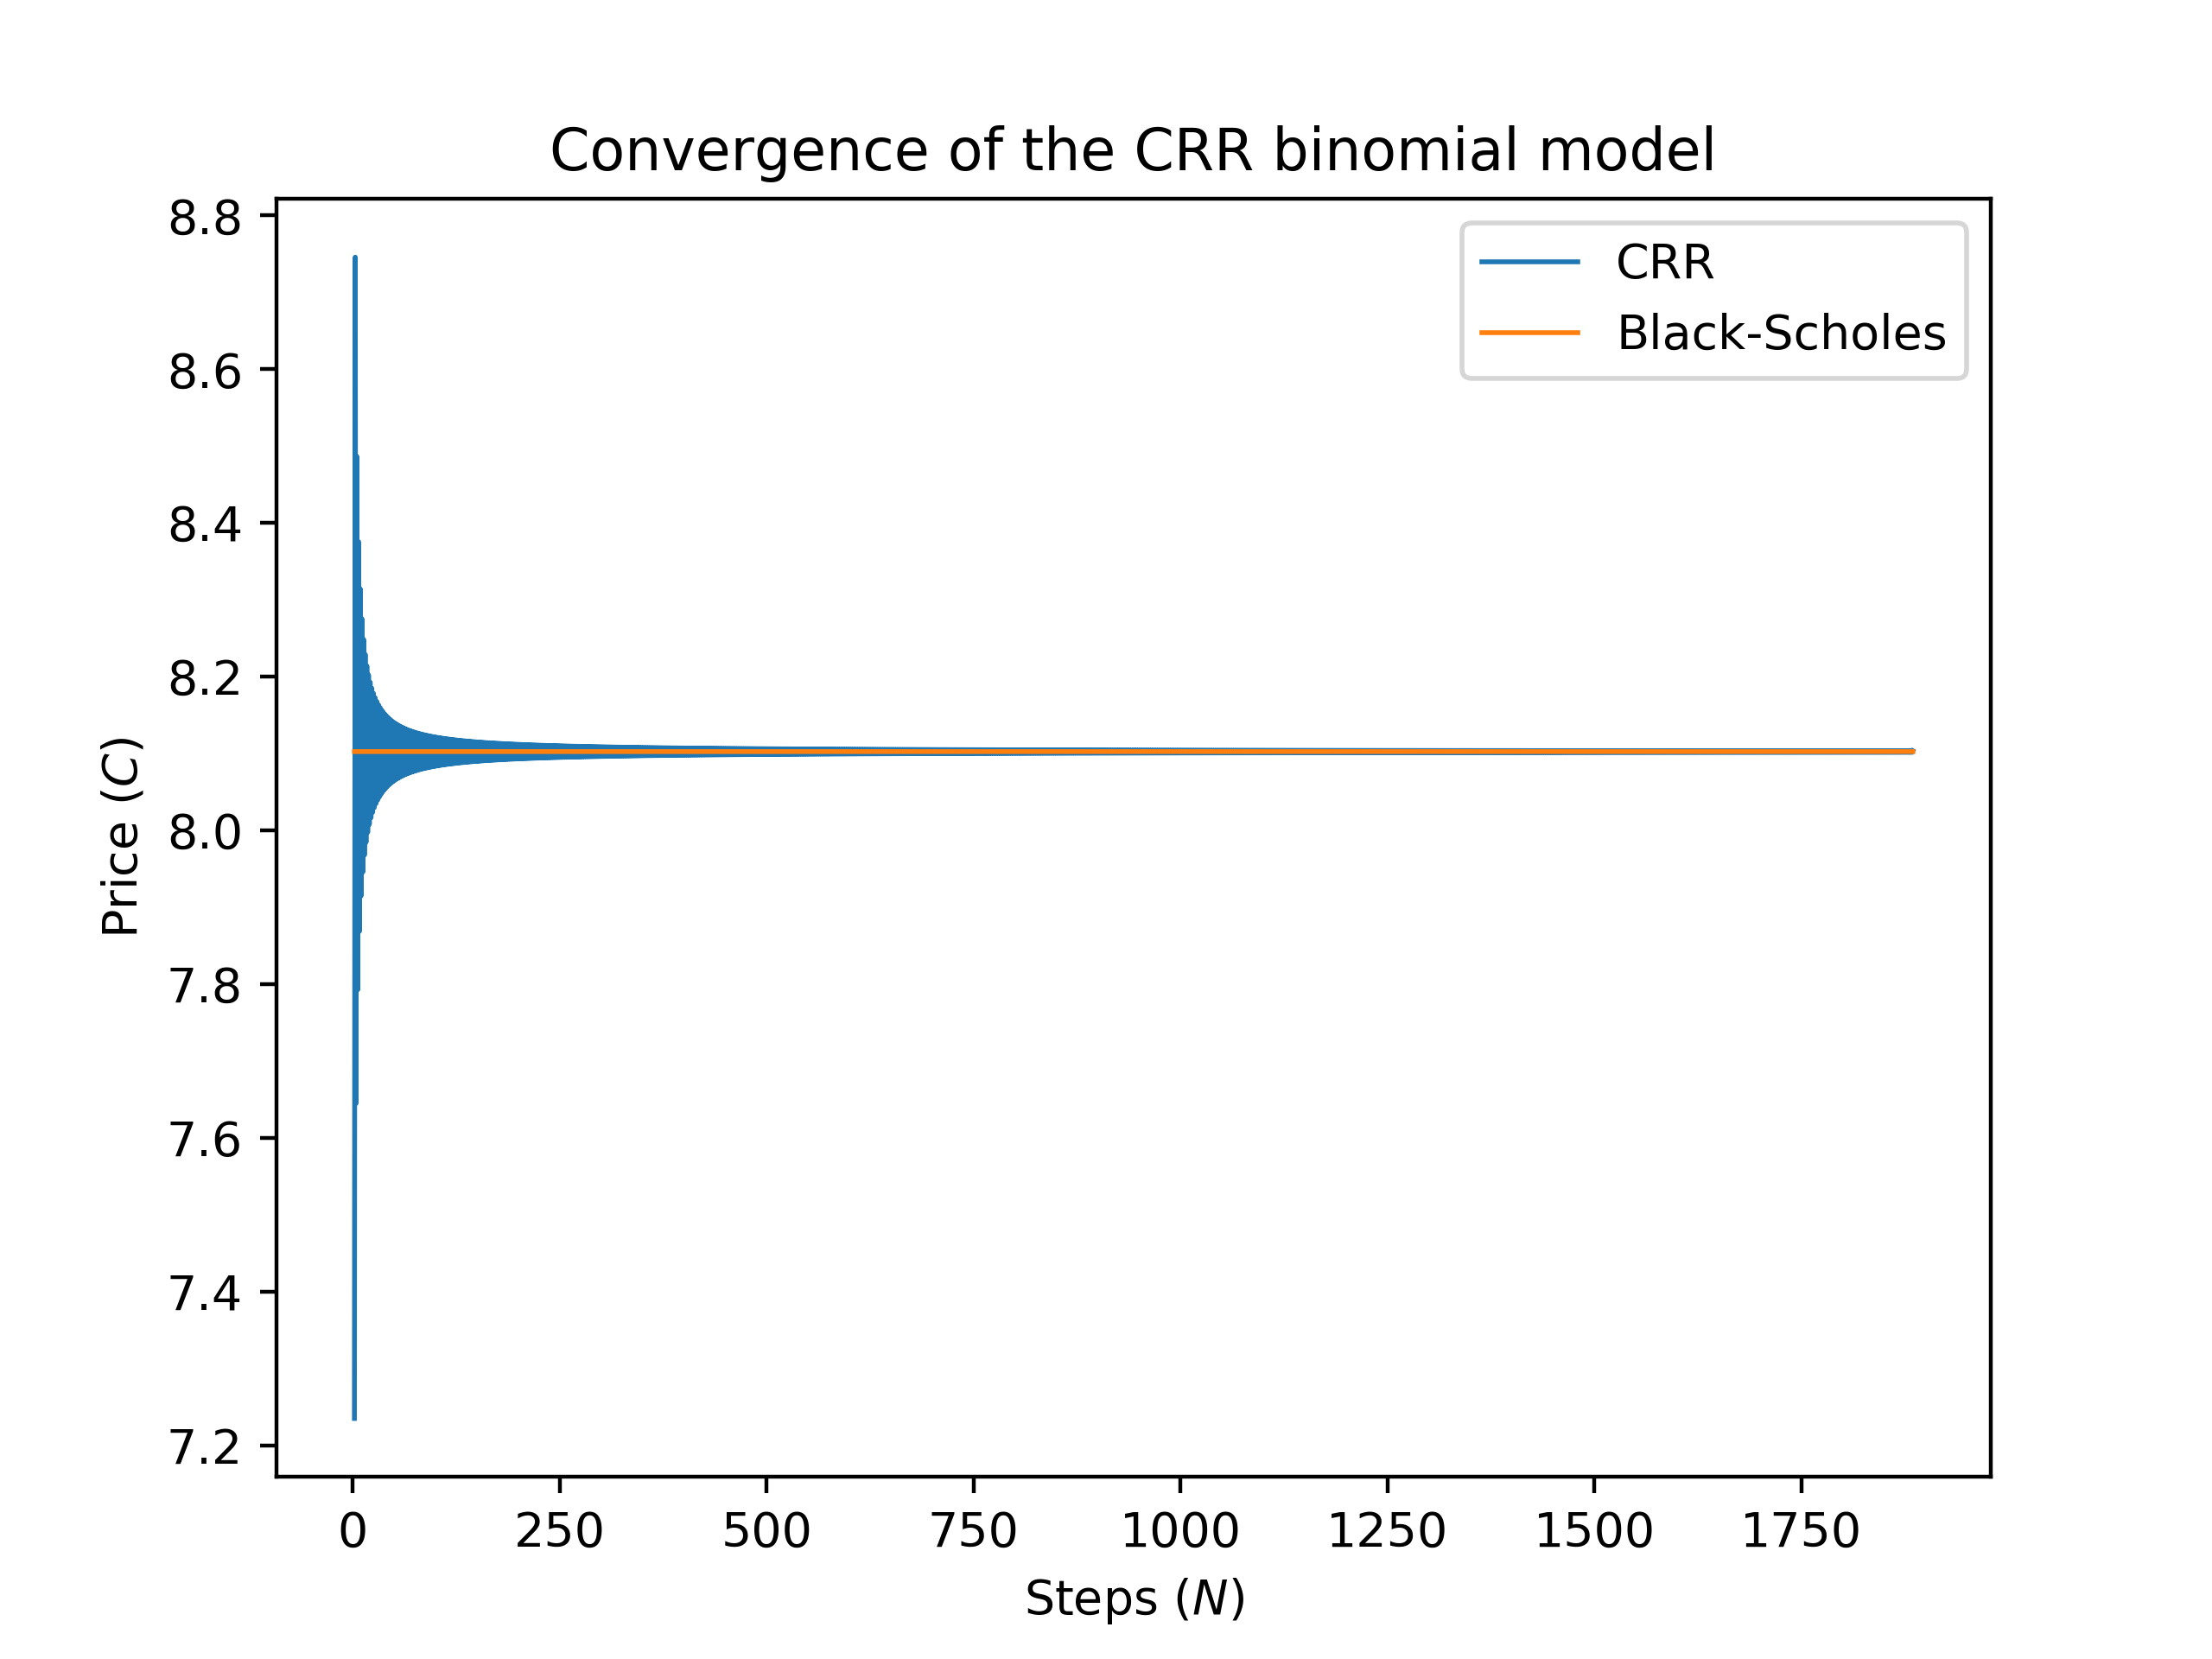
\includegraphics[width=75mm]{images/convergence.png}
	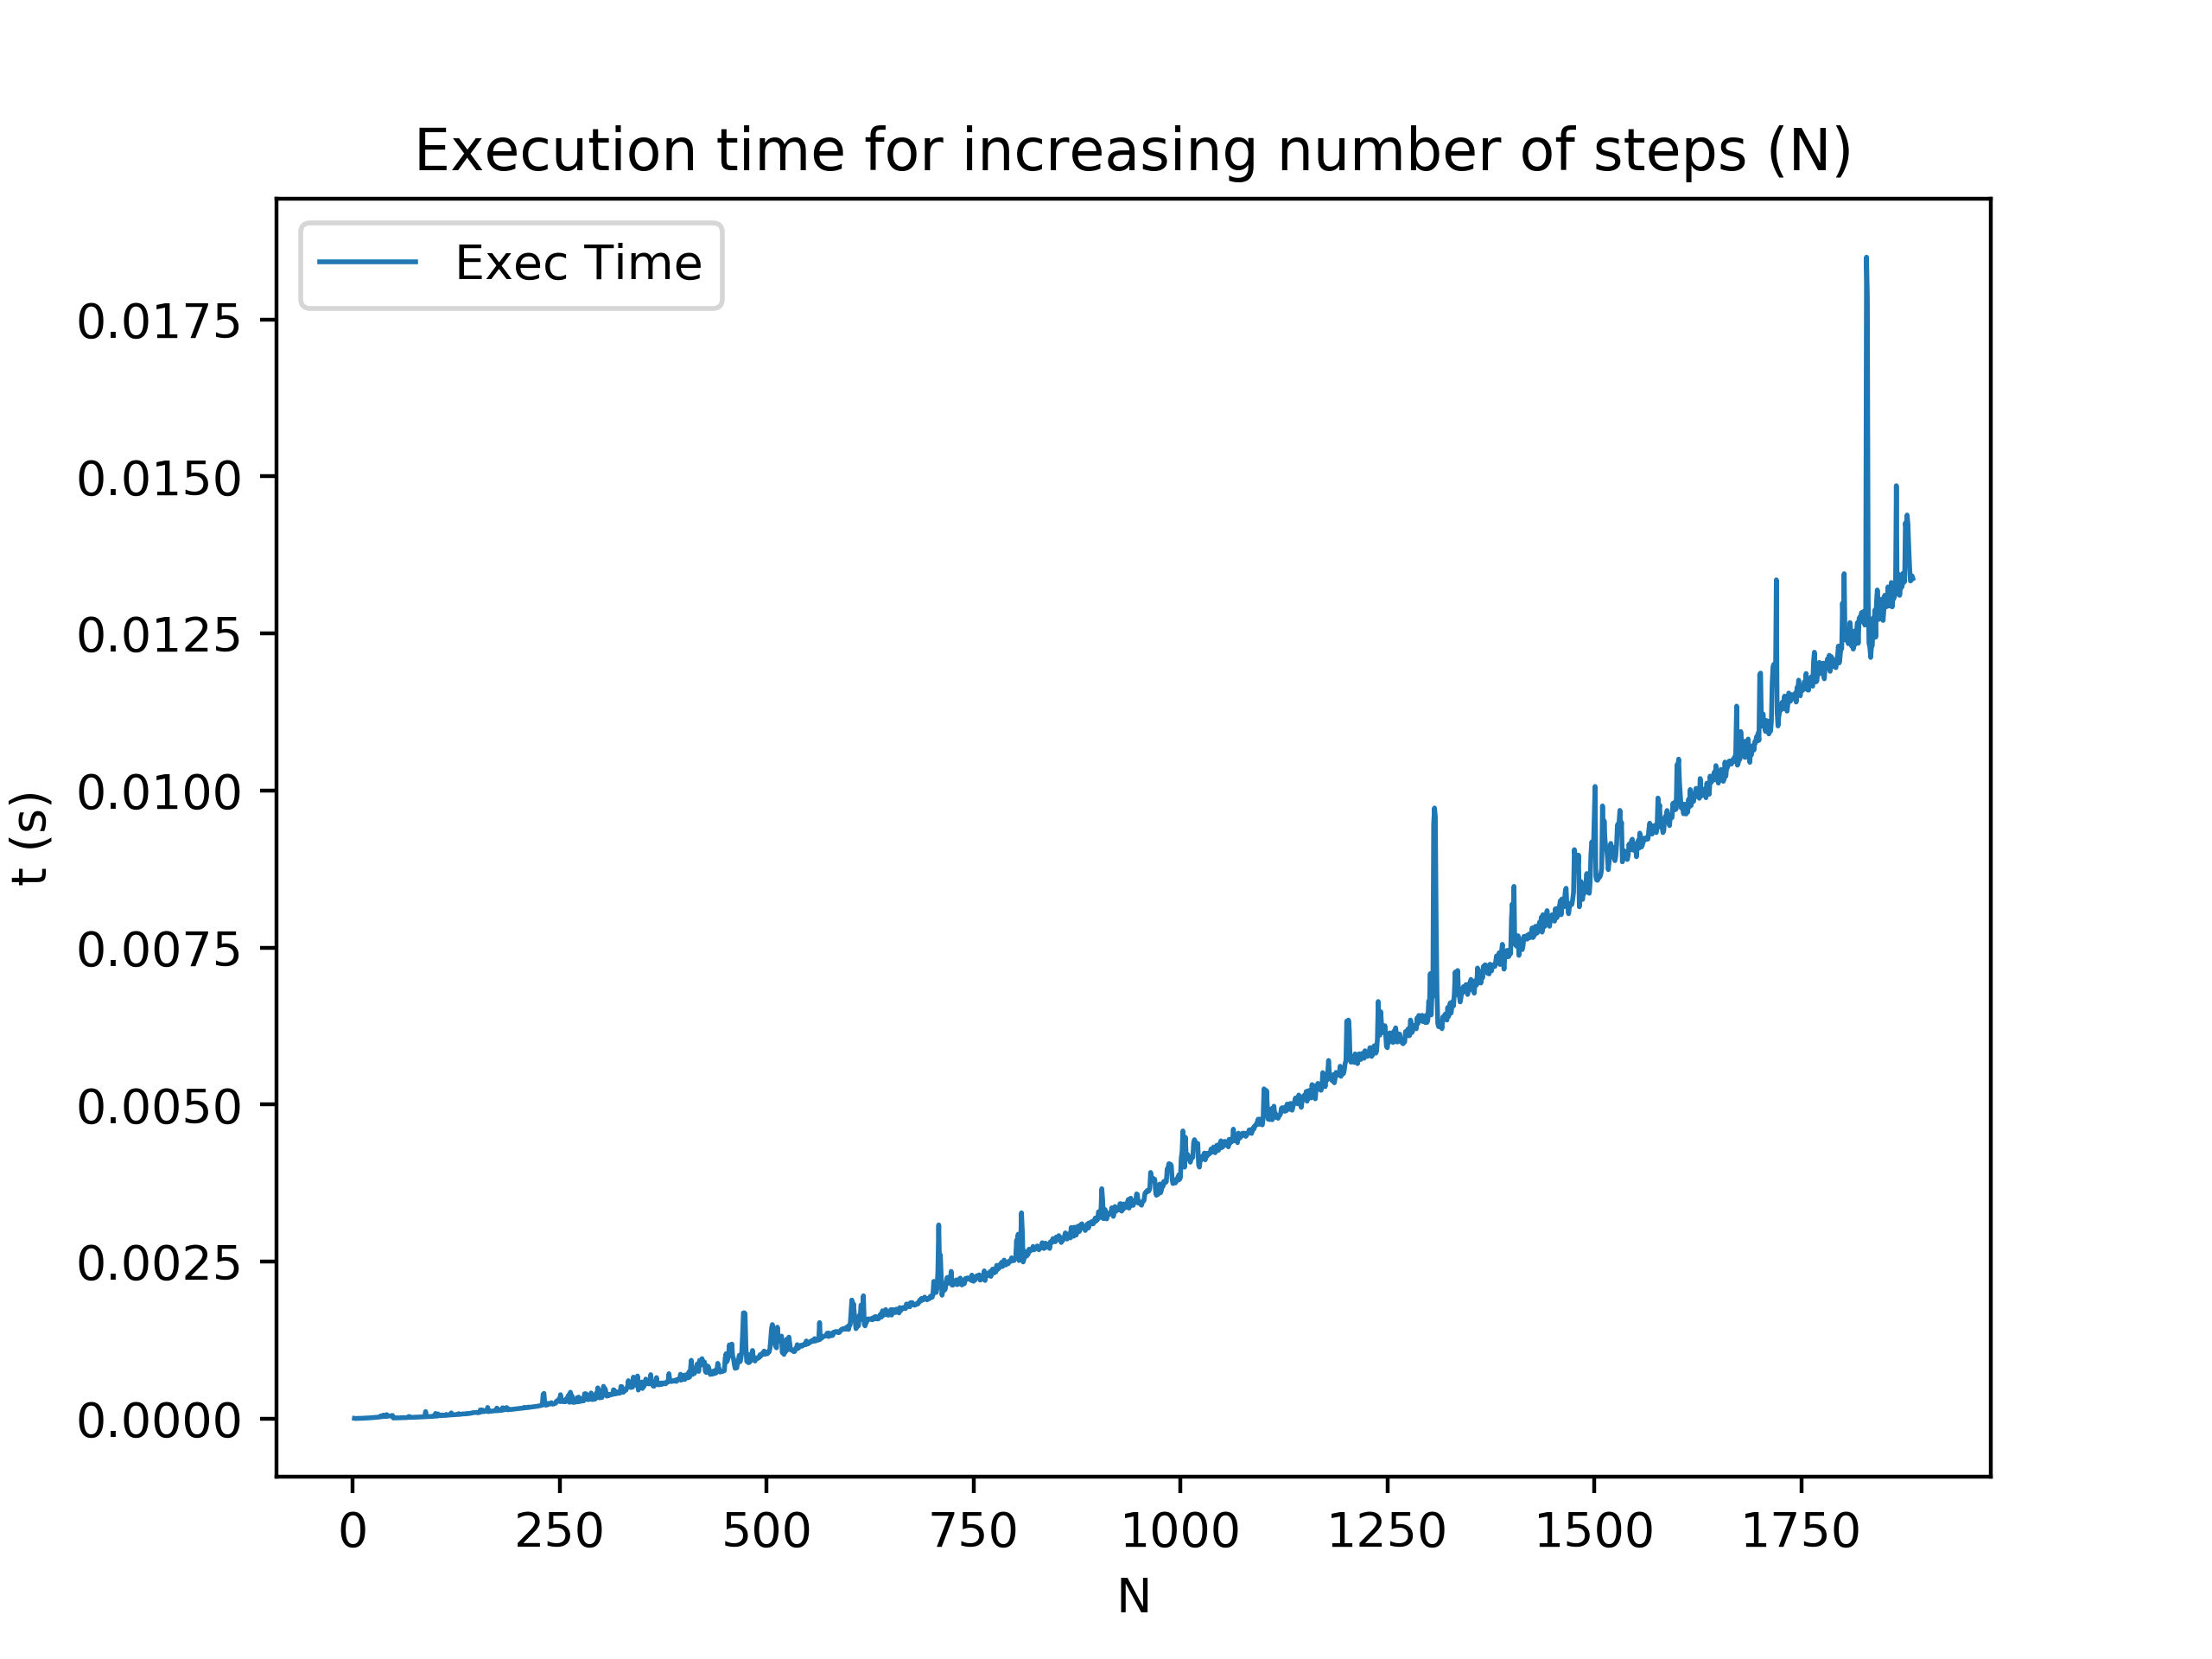
\includegraphics[width=75mm]{images/q2_time.png}
	\caption{CRR binomial option price as a function of number of steps $N$. The convergence is easily observable as $N$ grows.}
	\label{convergence}
\end{figure}

\section*{Question 3}

This question concerns pricing of an american put option with values $K = \$100.0, \ \sigma = 0.2, \ r = 5\%$. As the black \& scholes model is unapplicable on american options, the absolute error between the price calculated with $N$ steps and $N-1$ steps was used to make sure the required accuracy of $10^{-3}$ was met using the CRR binomial model. As indicated in the plot below, a maximum of approximately 2200 steps was needed to ensure the accuracy when time to maturity was set to 1 year. Therefore, $N=2250$ was used in the subsequent calculations in this question. The time complexity for increasing number of steps was found to be of magnitude $\mathcal{O}(N^2)$.

\begin{figure}[H]
	\centering
	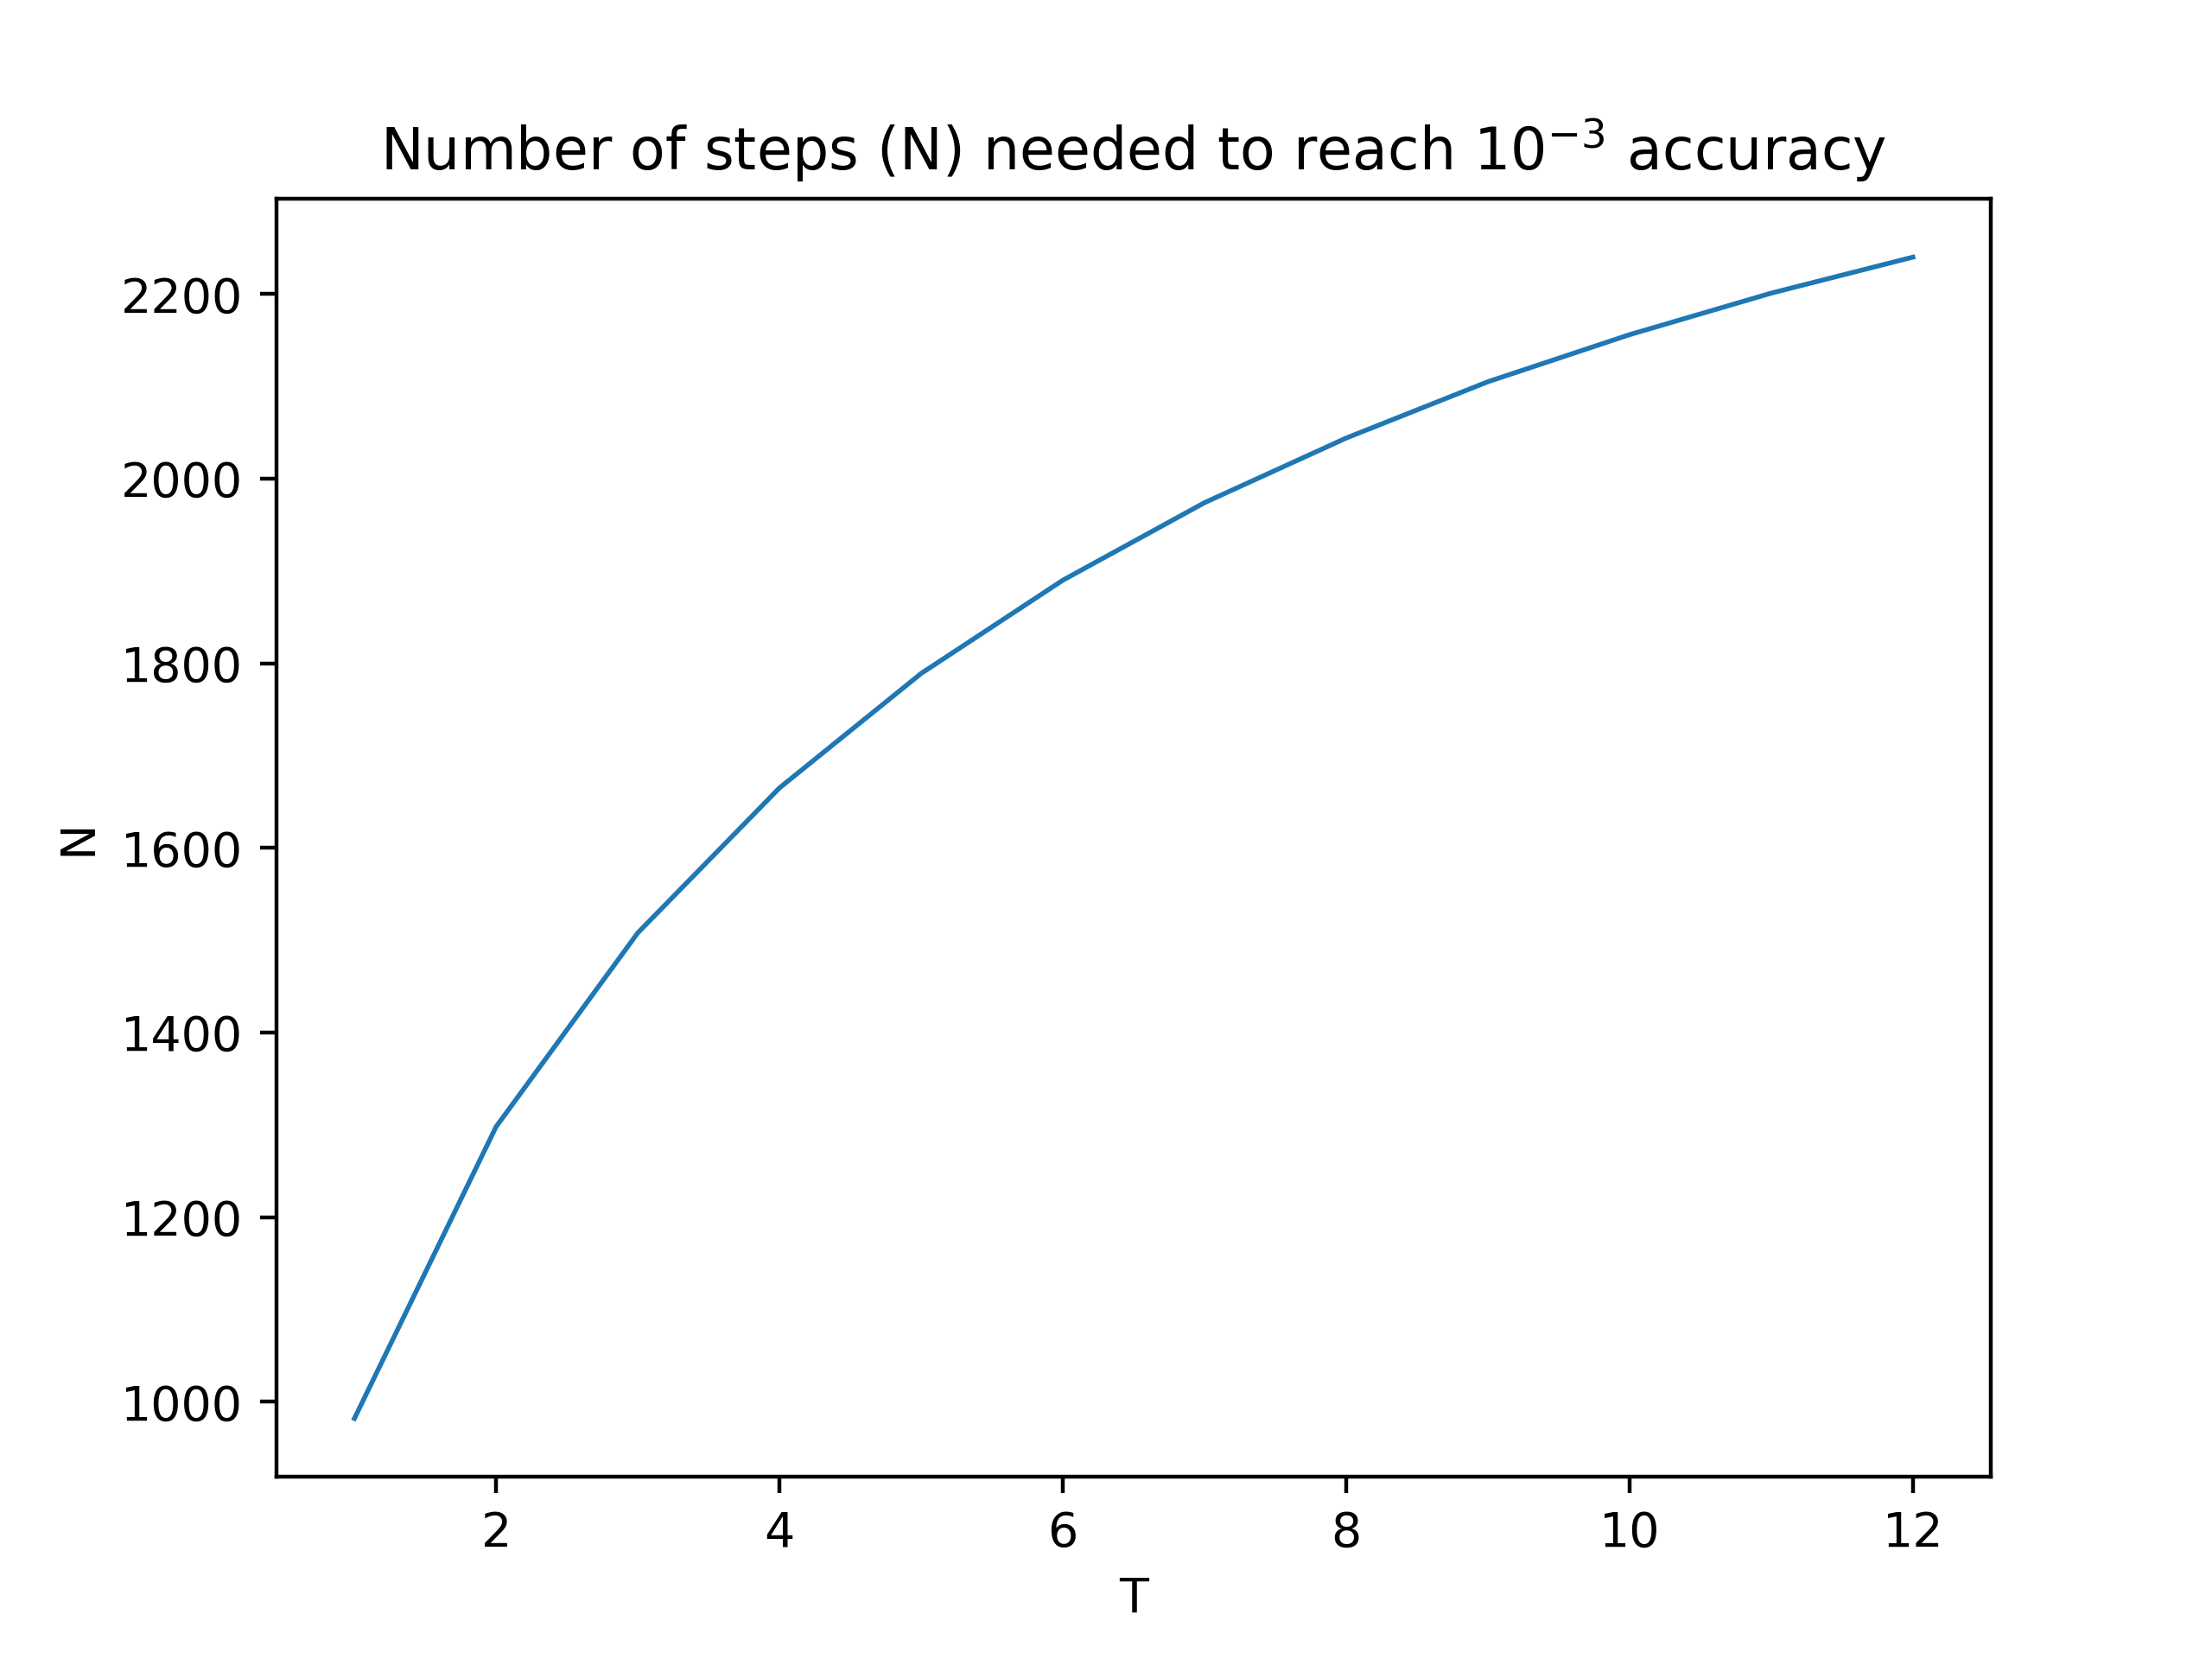
\includegraphics[width=75mm]{images/q3_n.png}
	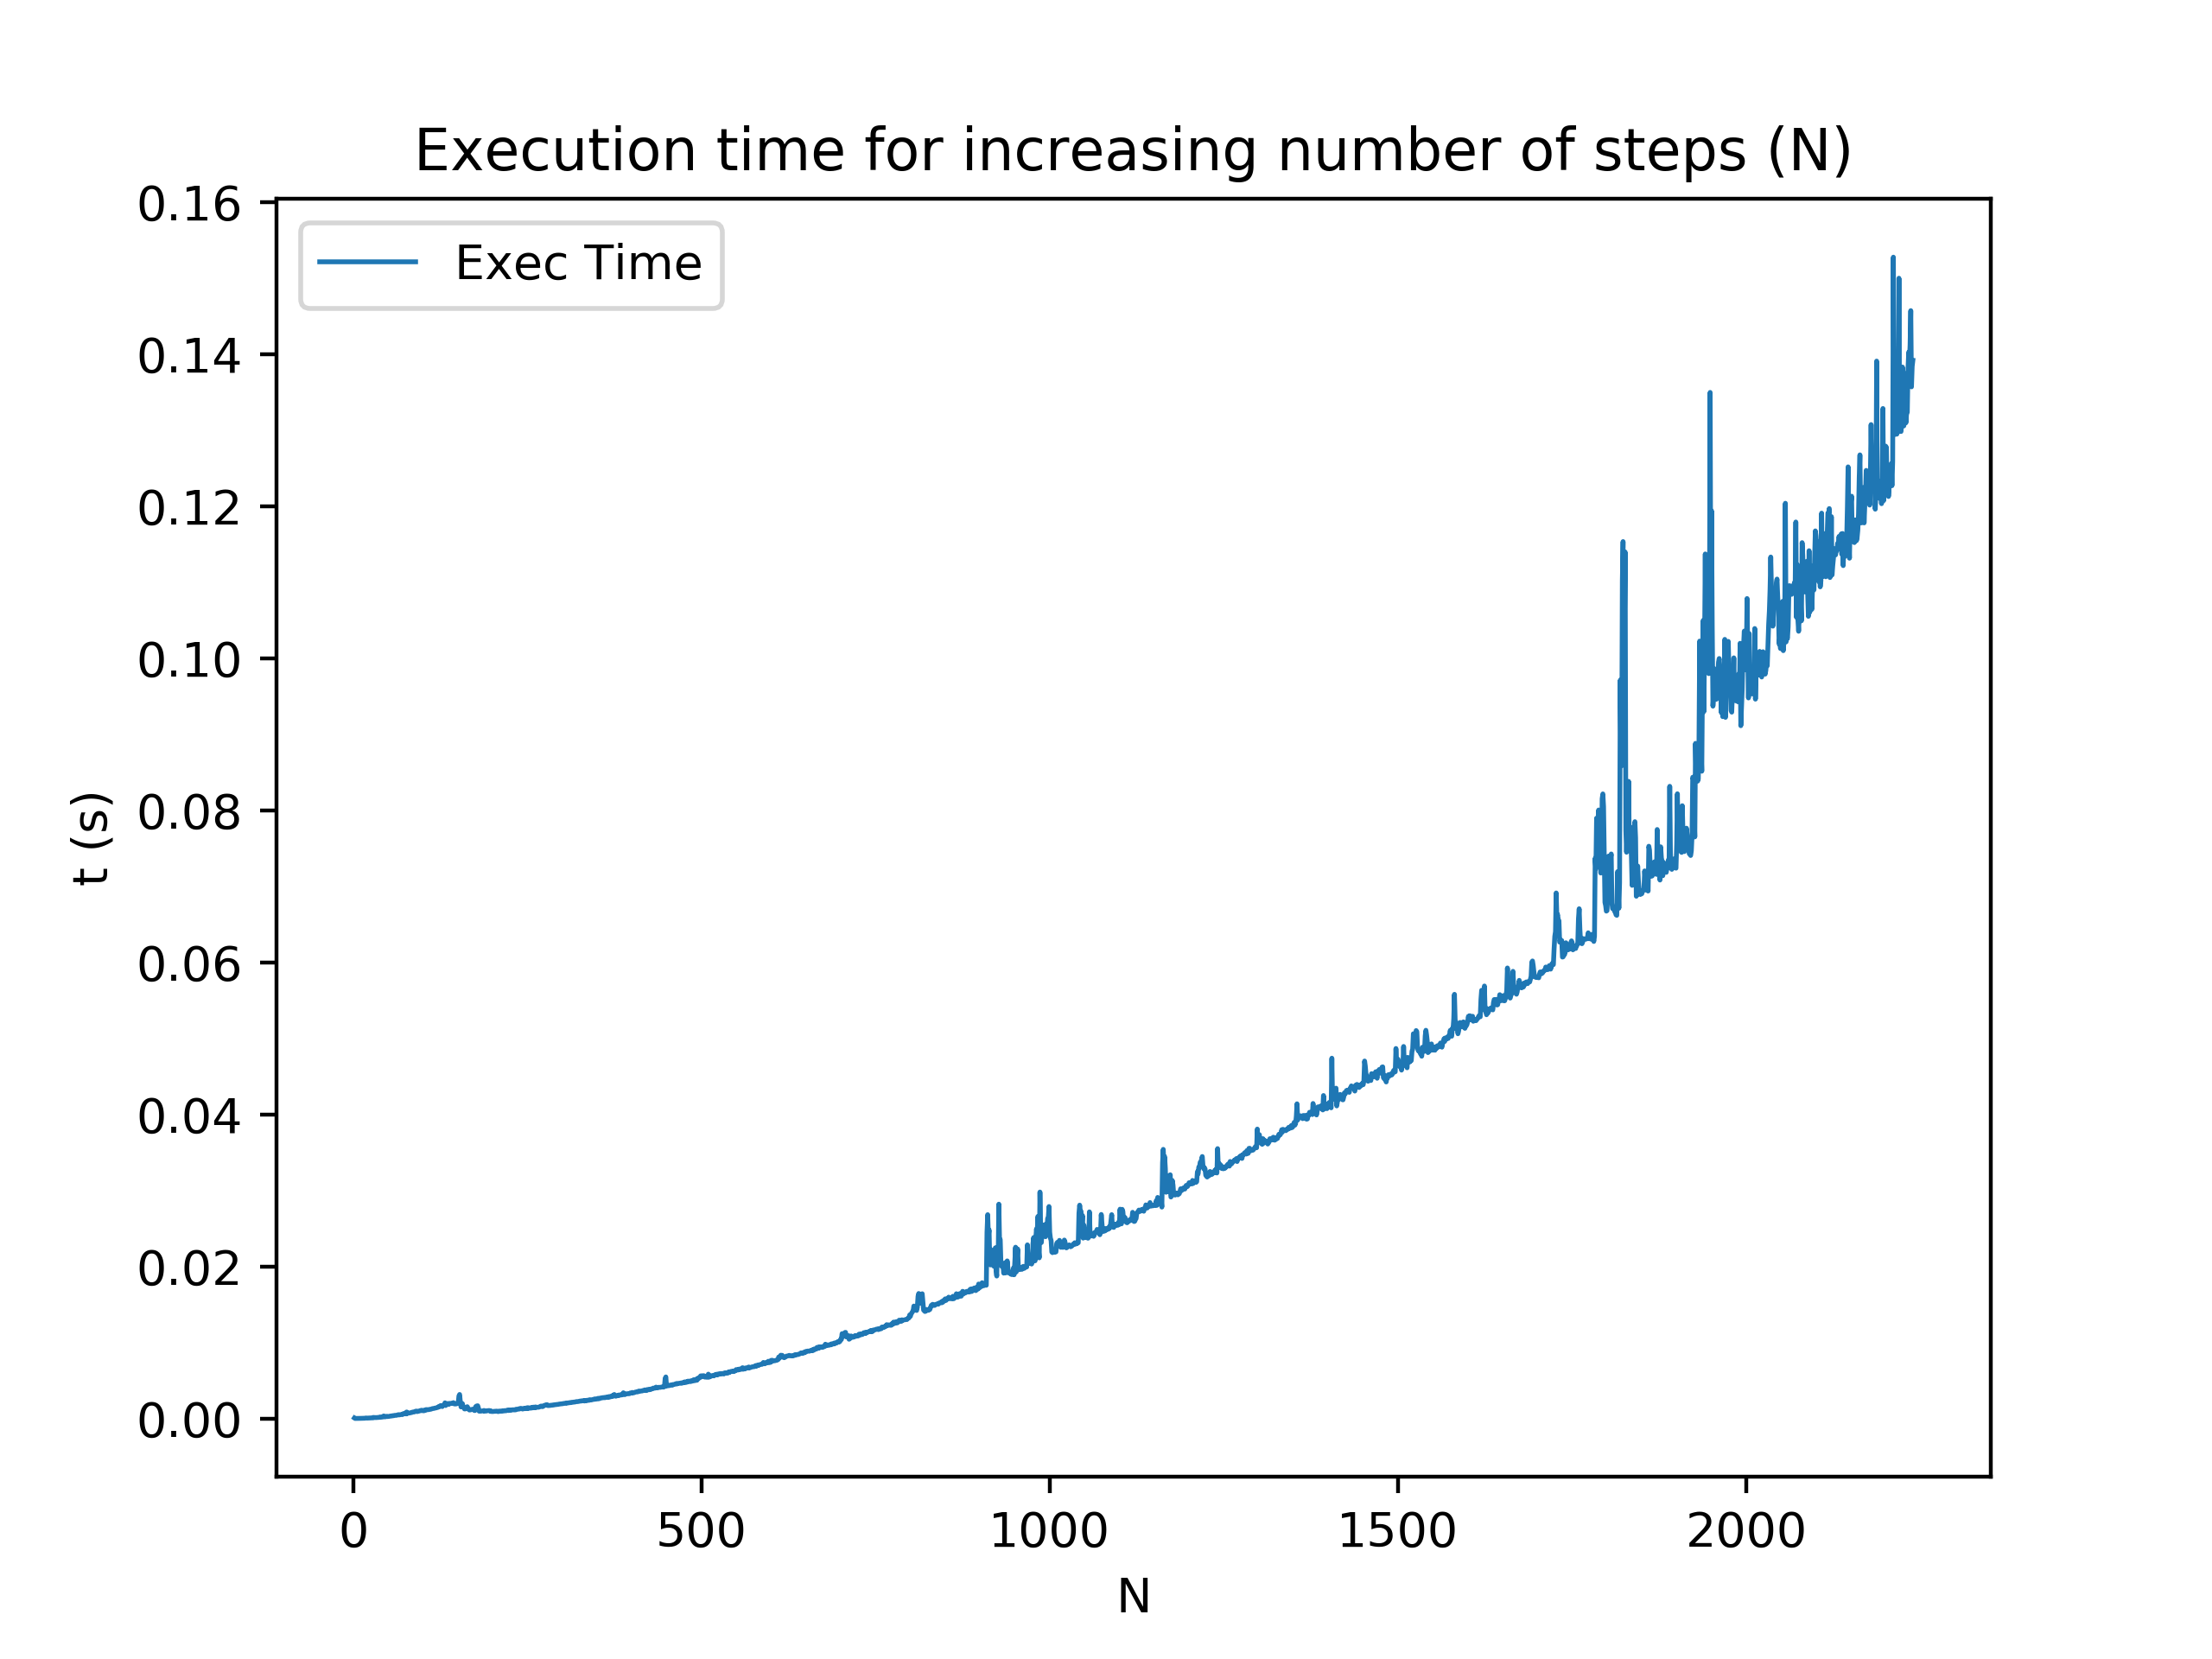
\includegraphics[width=75mm]{images/q3_time.png}
	\caption{To the left the number of steps needed to ensure an accuracy of $10^{-3}$ is shown as a function of $T$. To the right, the execution time as a function of the number of steps is shown.}
\end{figure}


\begin{figure}[H]
	\centering
	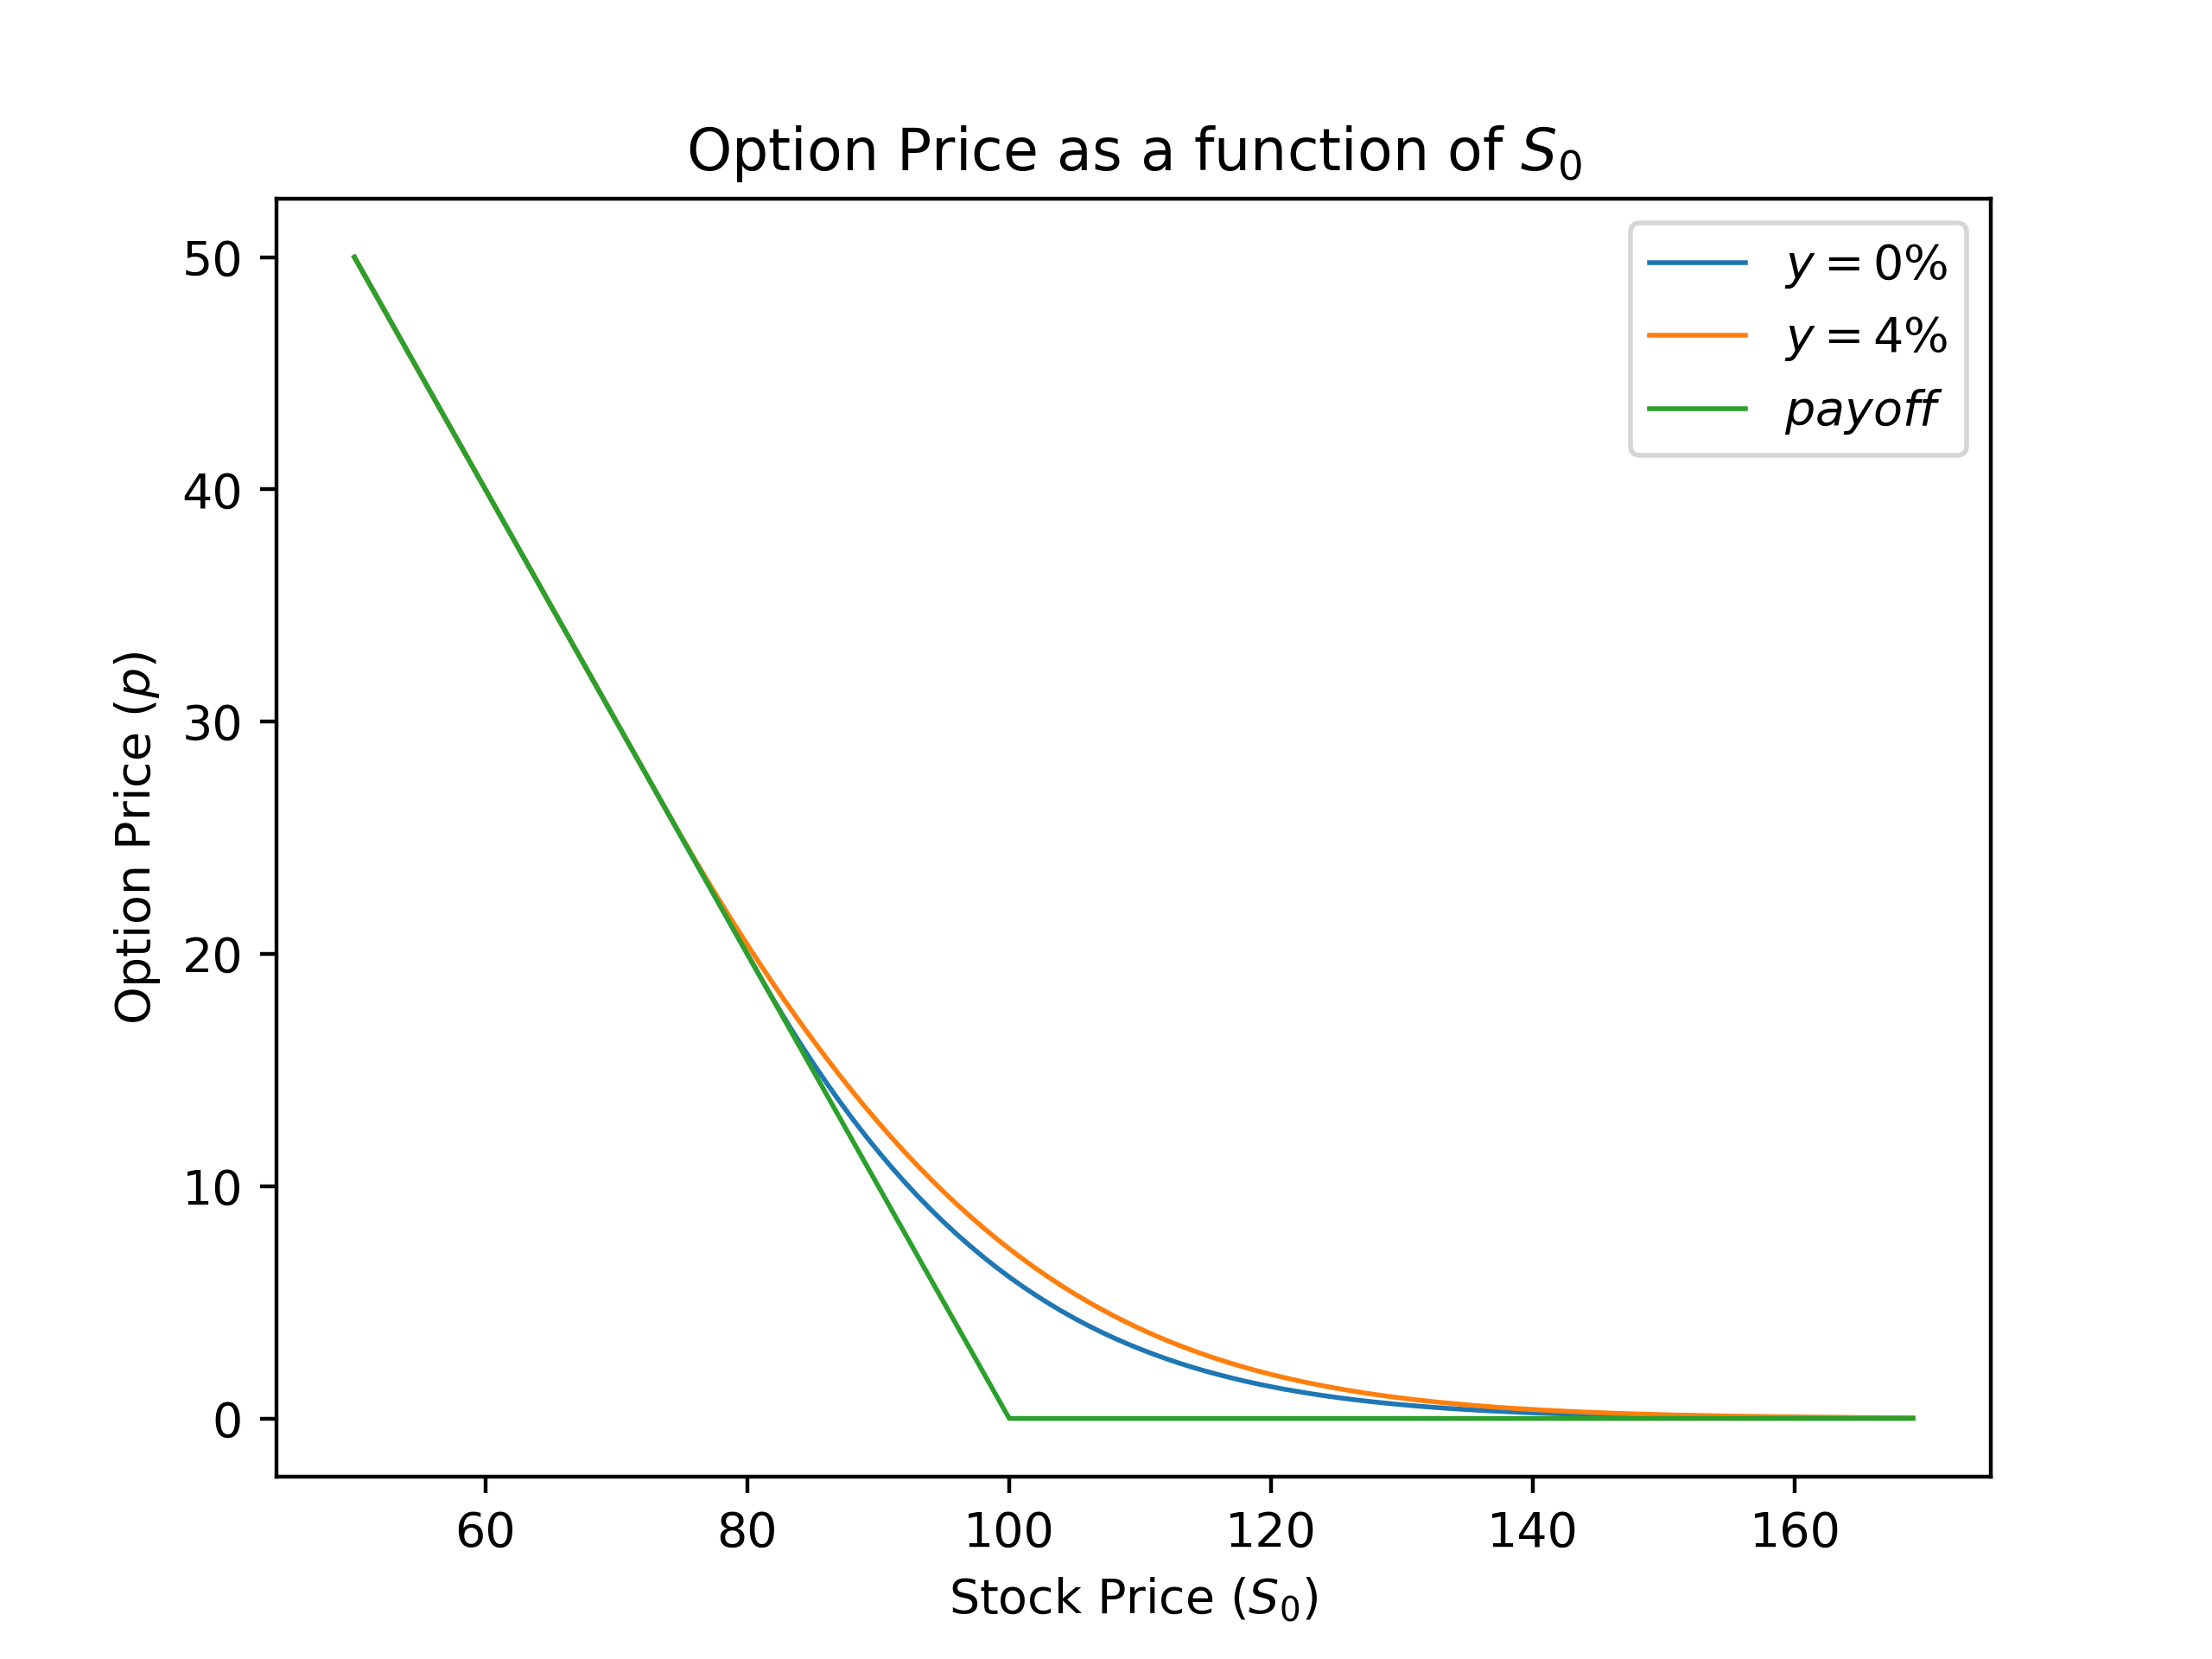
\includegraphics[width=90mm]{images/q3_function_of_S0.png}
	\caption{CRR binomial put price as a function of inital stock price $S_0$.}
	\label{q3S0}
\end{figure}

Figure \ref{q3S0} shows that when the initial stock price increases, the option price of the american put option also decreases. The strike price of the option is $\$100$, i.e gives the holder the right to sell a share of the underlying asset for $\$100$, and thus the option is less valuable for the holder the higher the initial stock price is and is thus prices lower. For low values of $S_0$ the price is equivalent to the the option intrinsic value due to the ability to exercise early. 

When the dividend yield increases, the price of the put option is higher. This is due to the fact that the value of the underlying asset decreases with the value of the dividend after the dividend date. As such the put option, giving the right to sell the asset at the strike price, increases in value when the dividend is increased and should thus be priced higher. This does however not hold for small values of $S_0$ as the option then is exercised earlier and thus still is priced according to the intrinsic value. 

\begin{figure}[H]
	\centering
	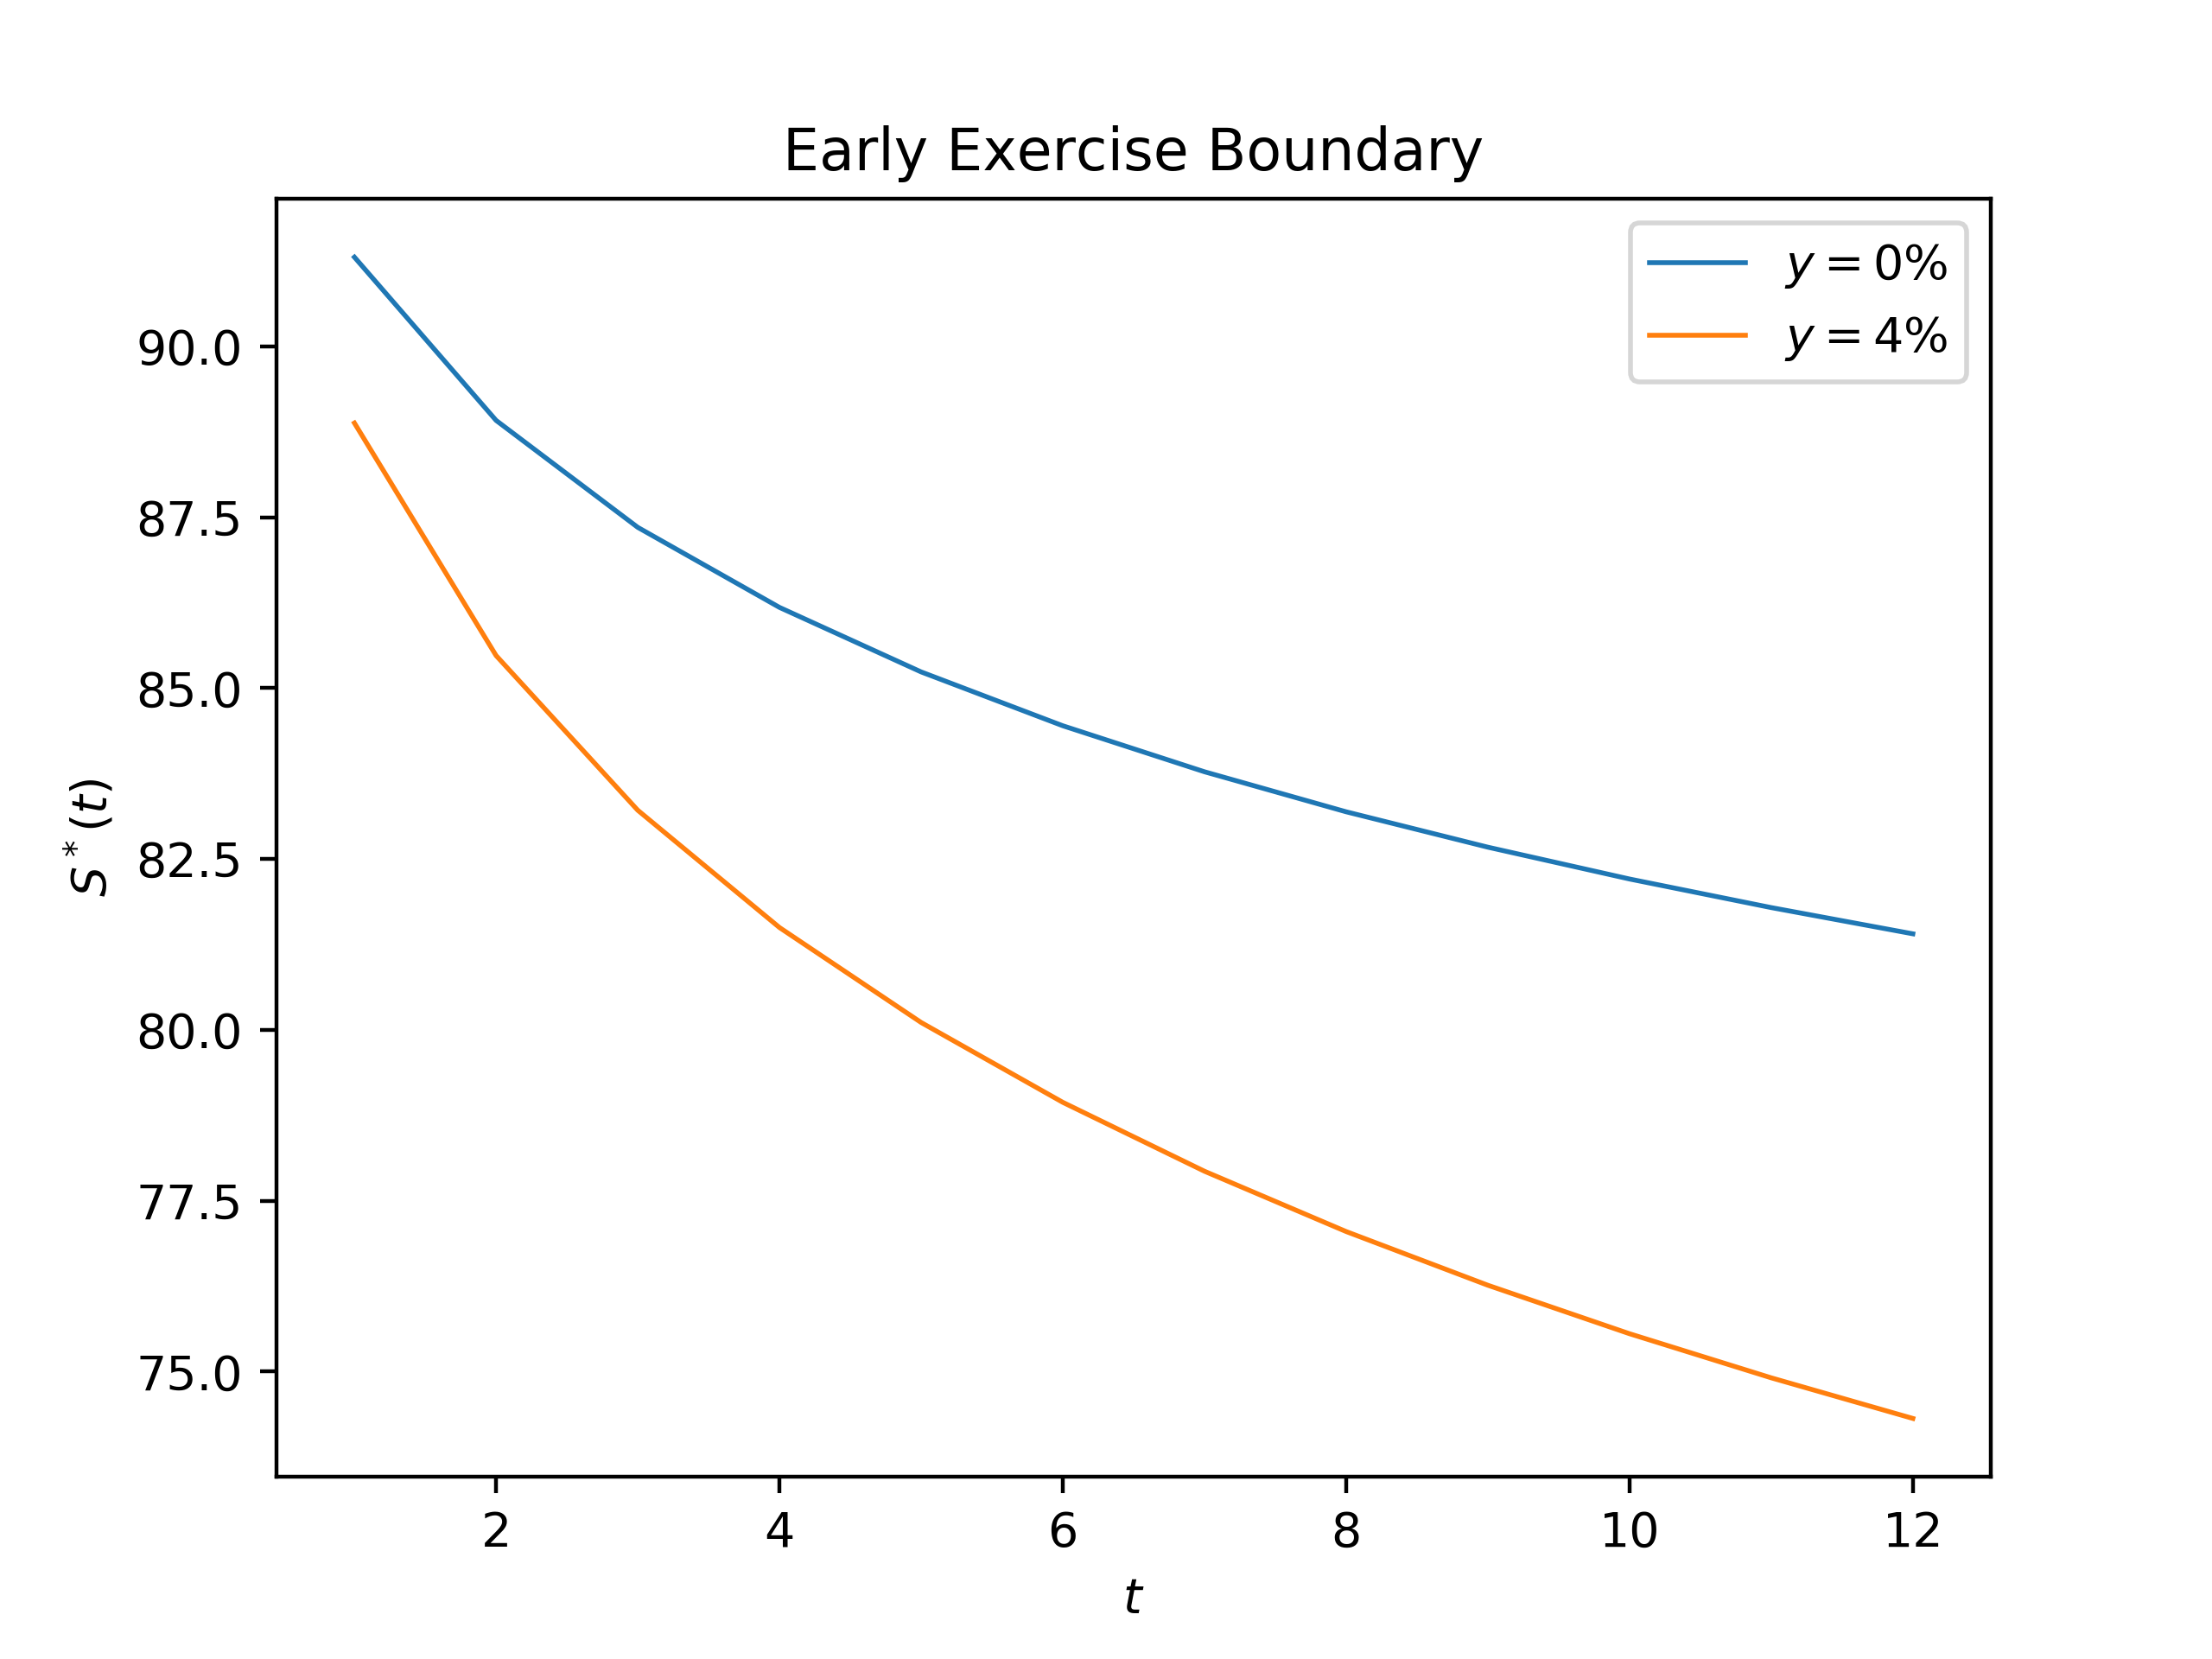
\includegraphics[width=90mm]{images/q3_critical.png}
	\caption{The critical price $S^*(t)$ as a function of time to maturity $t$ ranging from 1 month to 1 year.}
	\label{q3Crit}
\end{figure}

\begin{table}[H]
	\begin{center}
		\begin{tabular}{ || c | c | c ||}
		\hline
		T & $S^*$ ($q=0\%$) & $S^*$ ($q = 4\%$)\\ 
		\hline
		1.0 & 91.3068 & 88.88 \\
		2.0 & 88.9181 & 85.4771 \\
		3.0 & 87.3533 & 83.2141 \\
		4.0 & 86.1824 & 81.4987 \\
		5.0 & 85.2383 & 80.1091 \\
		6.0 & 84.4505 & 78.9409 \\
		7.0 & 83.7774 & 77.9327 \\
		8.0 & 83.1916 & 77.0503 \\
		9.0 & 82.6741 & 76.2648 \\
		10.0 & 82.2084 & 75.5554 \\
		11.0 & 81.7902 & 74.9102 \\
		12.0 & 81.4064 & 74.3158 \\
		\hline 
		\end{tabular}
	\end{center}
	\caption{asd}
	\label{q3table}
\end{table}

For time to maturity ranging from 1 to 12 months, the critical price $S^*$ was numerically approximated by calculating the difference between the option price and the intrinsic value of the option for decreasing values of $S_0$. This was done with a step size of 1 until an lower bound was found at which the difference exceeded 0.005. The interval was then updated and the step size was divided by 10. The process was repeated until the step size was 0.0001. At this point the approximation of $S^*$, i.e. the highest value of the stock price that provided a difference less than 0.005, was well within the required tolerance. The results are presented in the plot and table above. (See Appendix \ref{critical} for more details on the algorithm used) 

Figure \ref{q3Crit} and table \ref{q3table} show the critical prices $S^*$ on the early exercise boundary as a function of time to maturity t (1-12 months). As the yield is increased from $0\%$ to $4\%$ the corresponding critical prices decrease. The reason for this is that the increase in dividend yield decreases the future price of the underlying asset, and thus makes it more profitable to hold the put option as time progresses. Because of this the time value of the option increases and thus the intrinsic value of the option has to be higher in order for a early exercise to be optimal. The intrinsic value increases as the stock price decreases and therefore the critical prices on the early exercise boundary are lower. 

\section*{Question 4}

This question concerns pricing of an american call option with values $K = \$100.0, \ \sigma = 0.2, \ r = 5\%$. As the black \& scholes model is unapplicable on american options, the absolute error between the price calculated with $N$ steps and $N-1$ steps was used to make sure the required accuracy of $10^{-3}$ was met using the CRR binomial model. As indicated in the plot below, a maximum of approximately 3780 steps was needed to ensure the accuracy when time to maturity was set to 1 year. Therefore, $N=3800$ was used in the subsequent calculations in this question. The time complexity for increasing number of steps was found to be of magnitude $\mathcal{O}(N^2)$.

\begin{figure}[H]
	\centering
	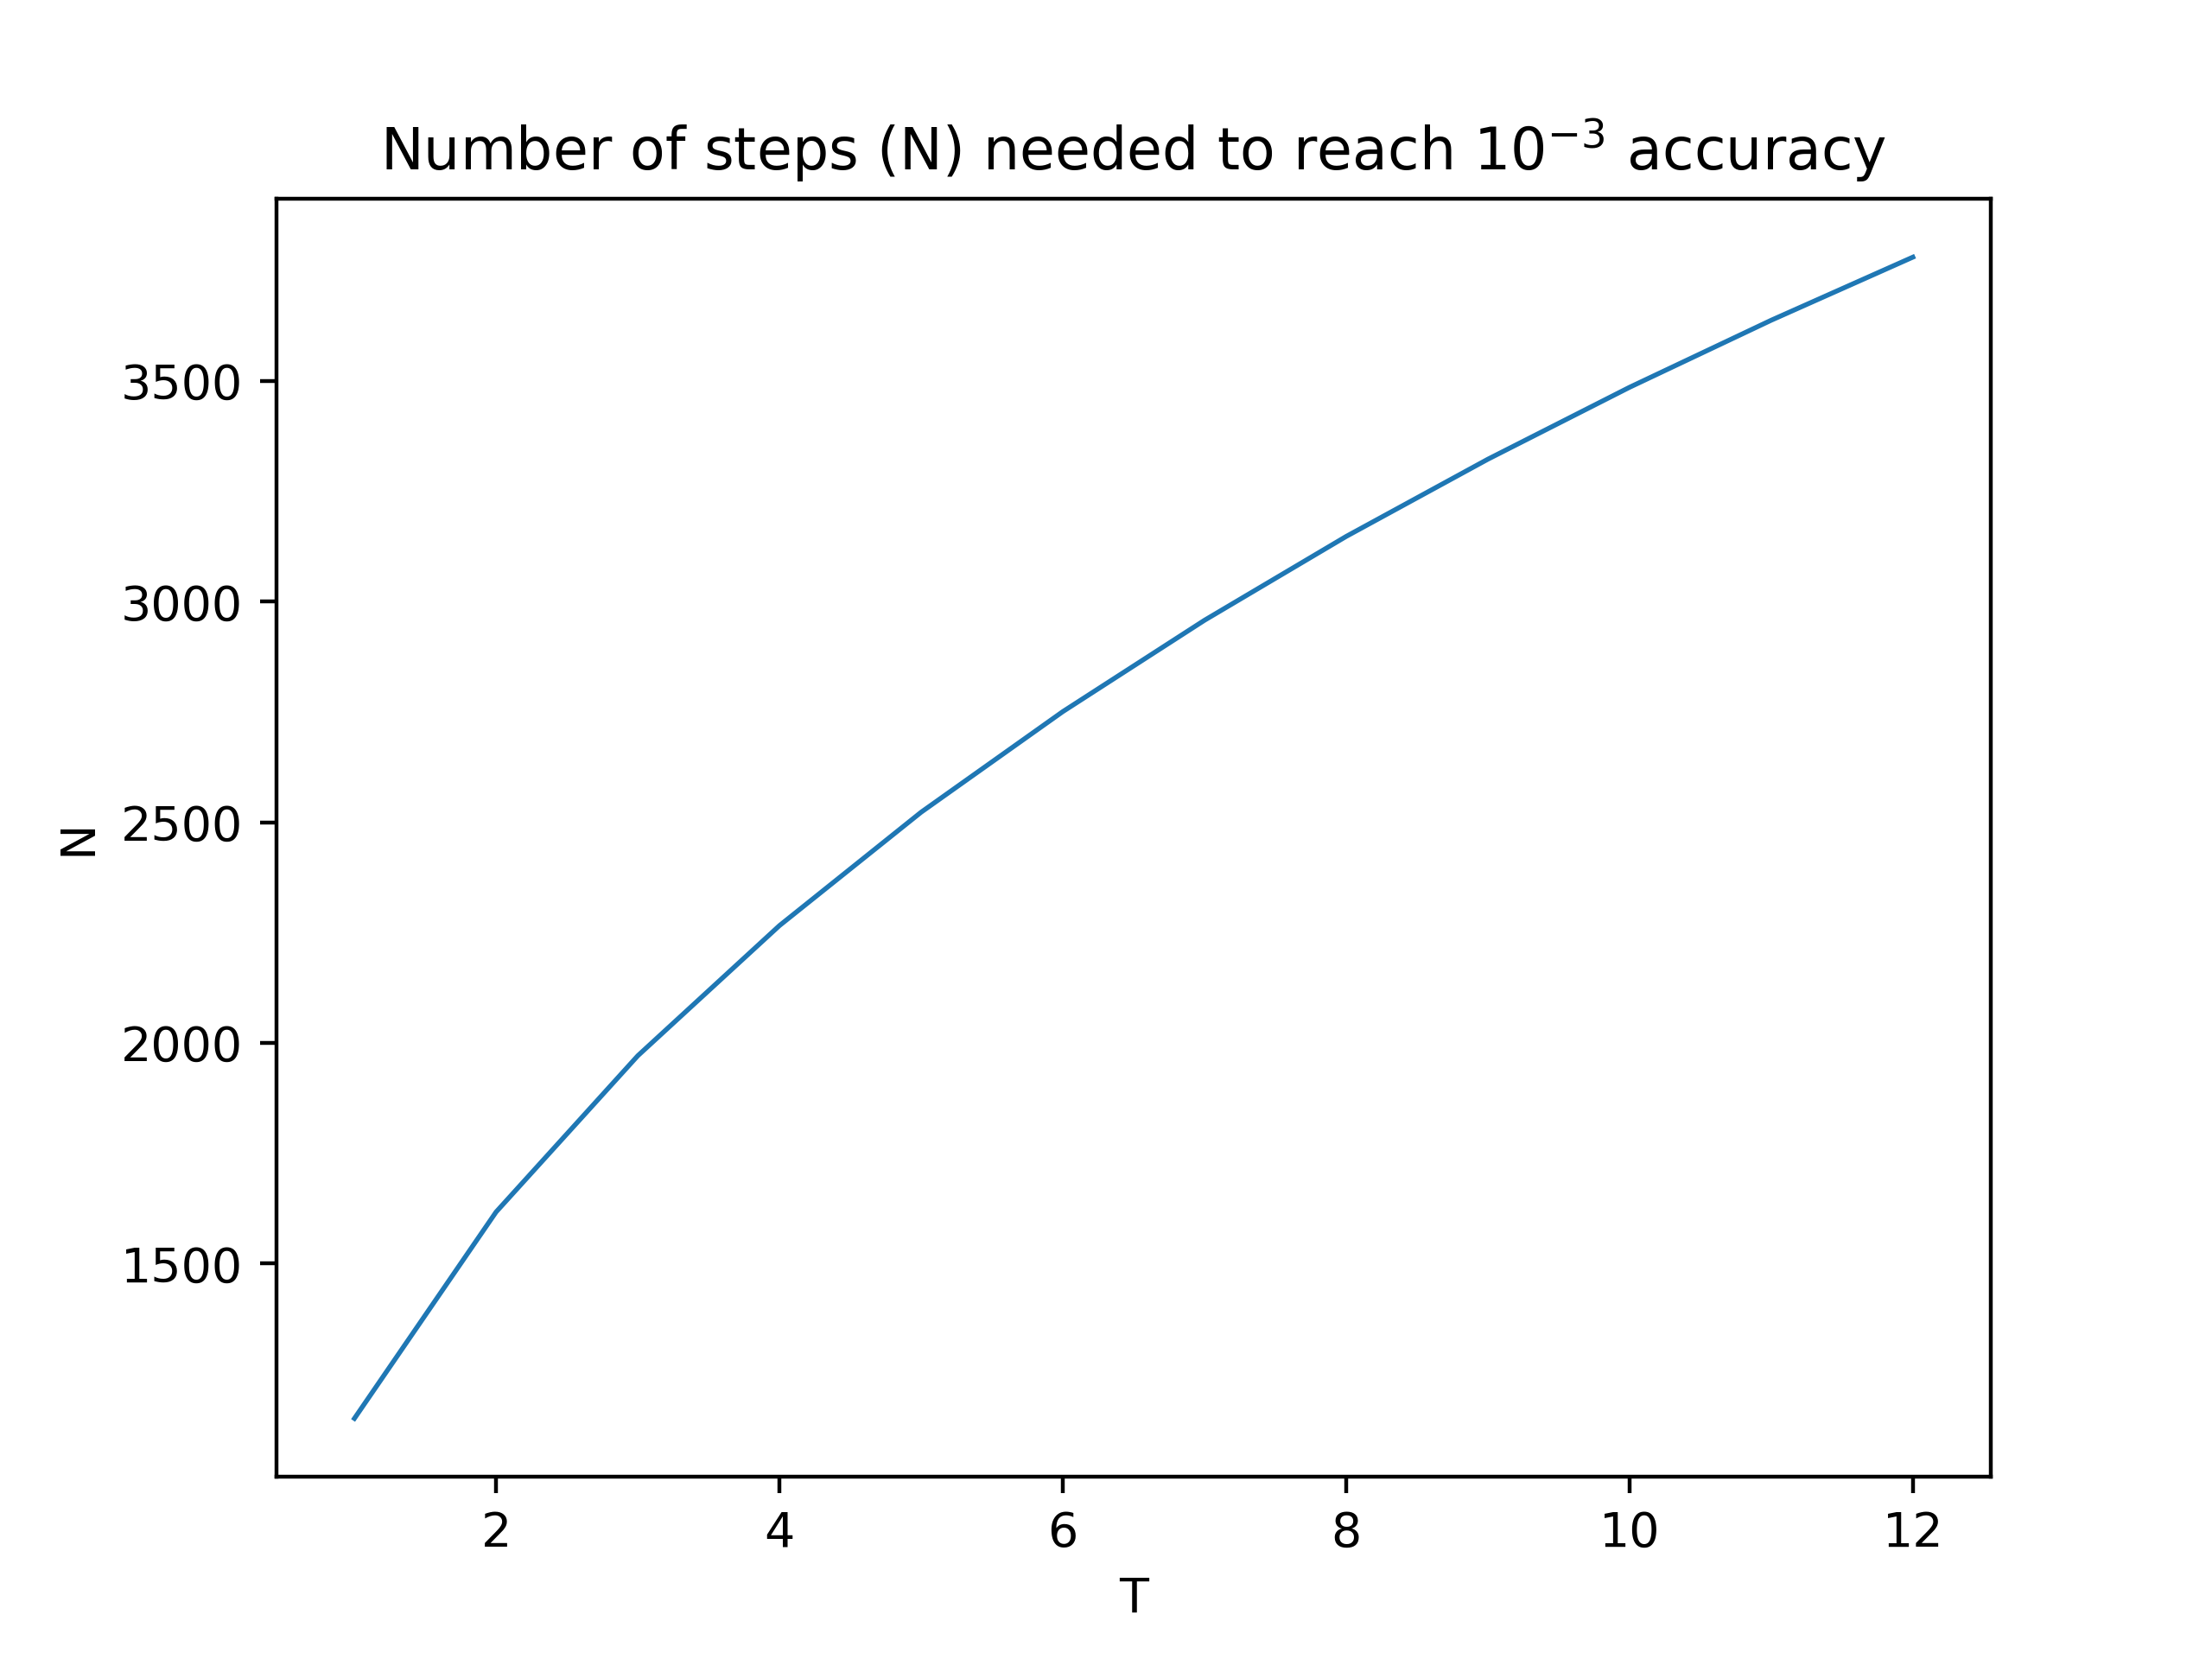
\includegraphics[width=75mm]{images/q4_n.png}
	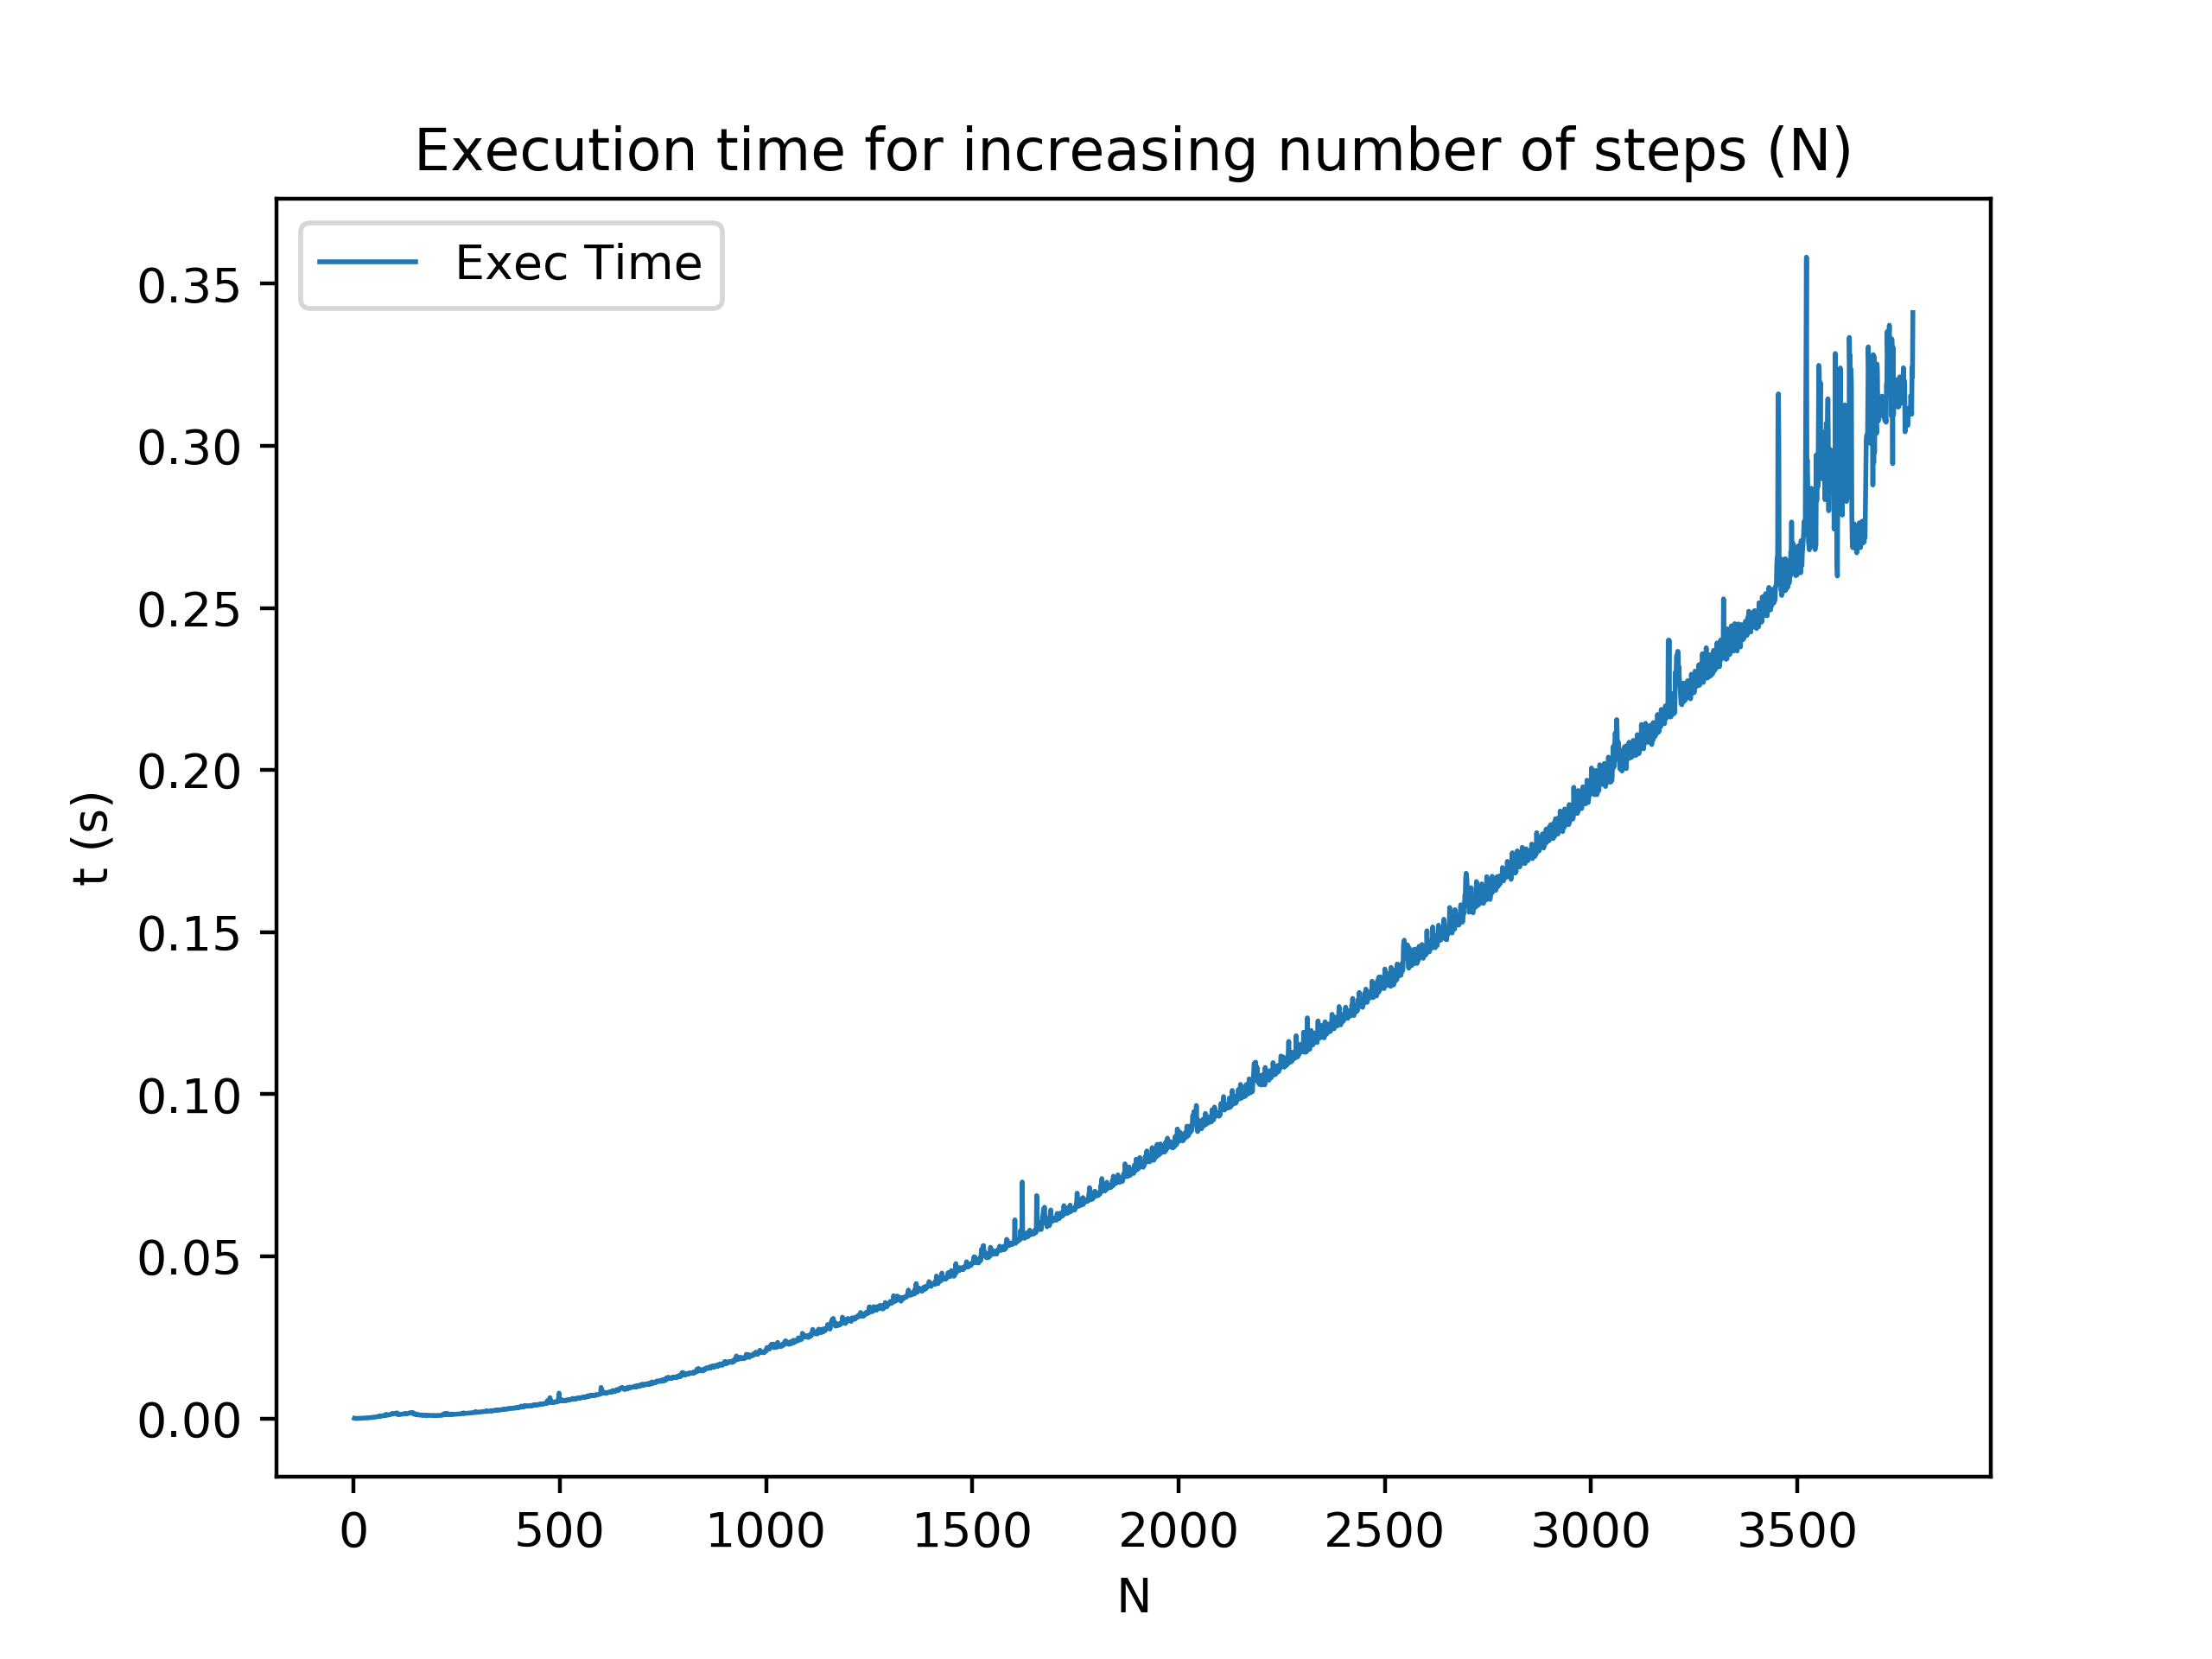
\includegraphics[width=75mm]{images/q4_time.png}
	\caption{To the left the number of steps needed to ensure an accuracy of $10^-3$ is shown as a function of $T$. To the right, the execution time as a function of the number of steps is shown.}
\end{figure}

\begin{figure}[H]
	\centering
	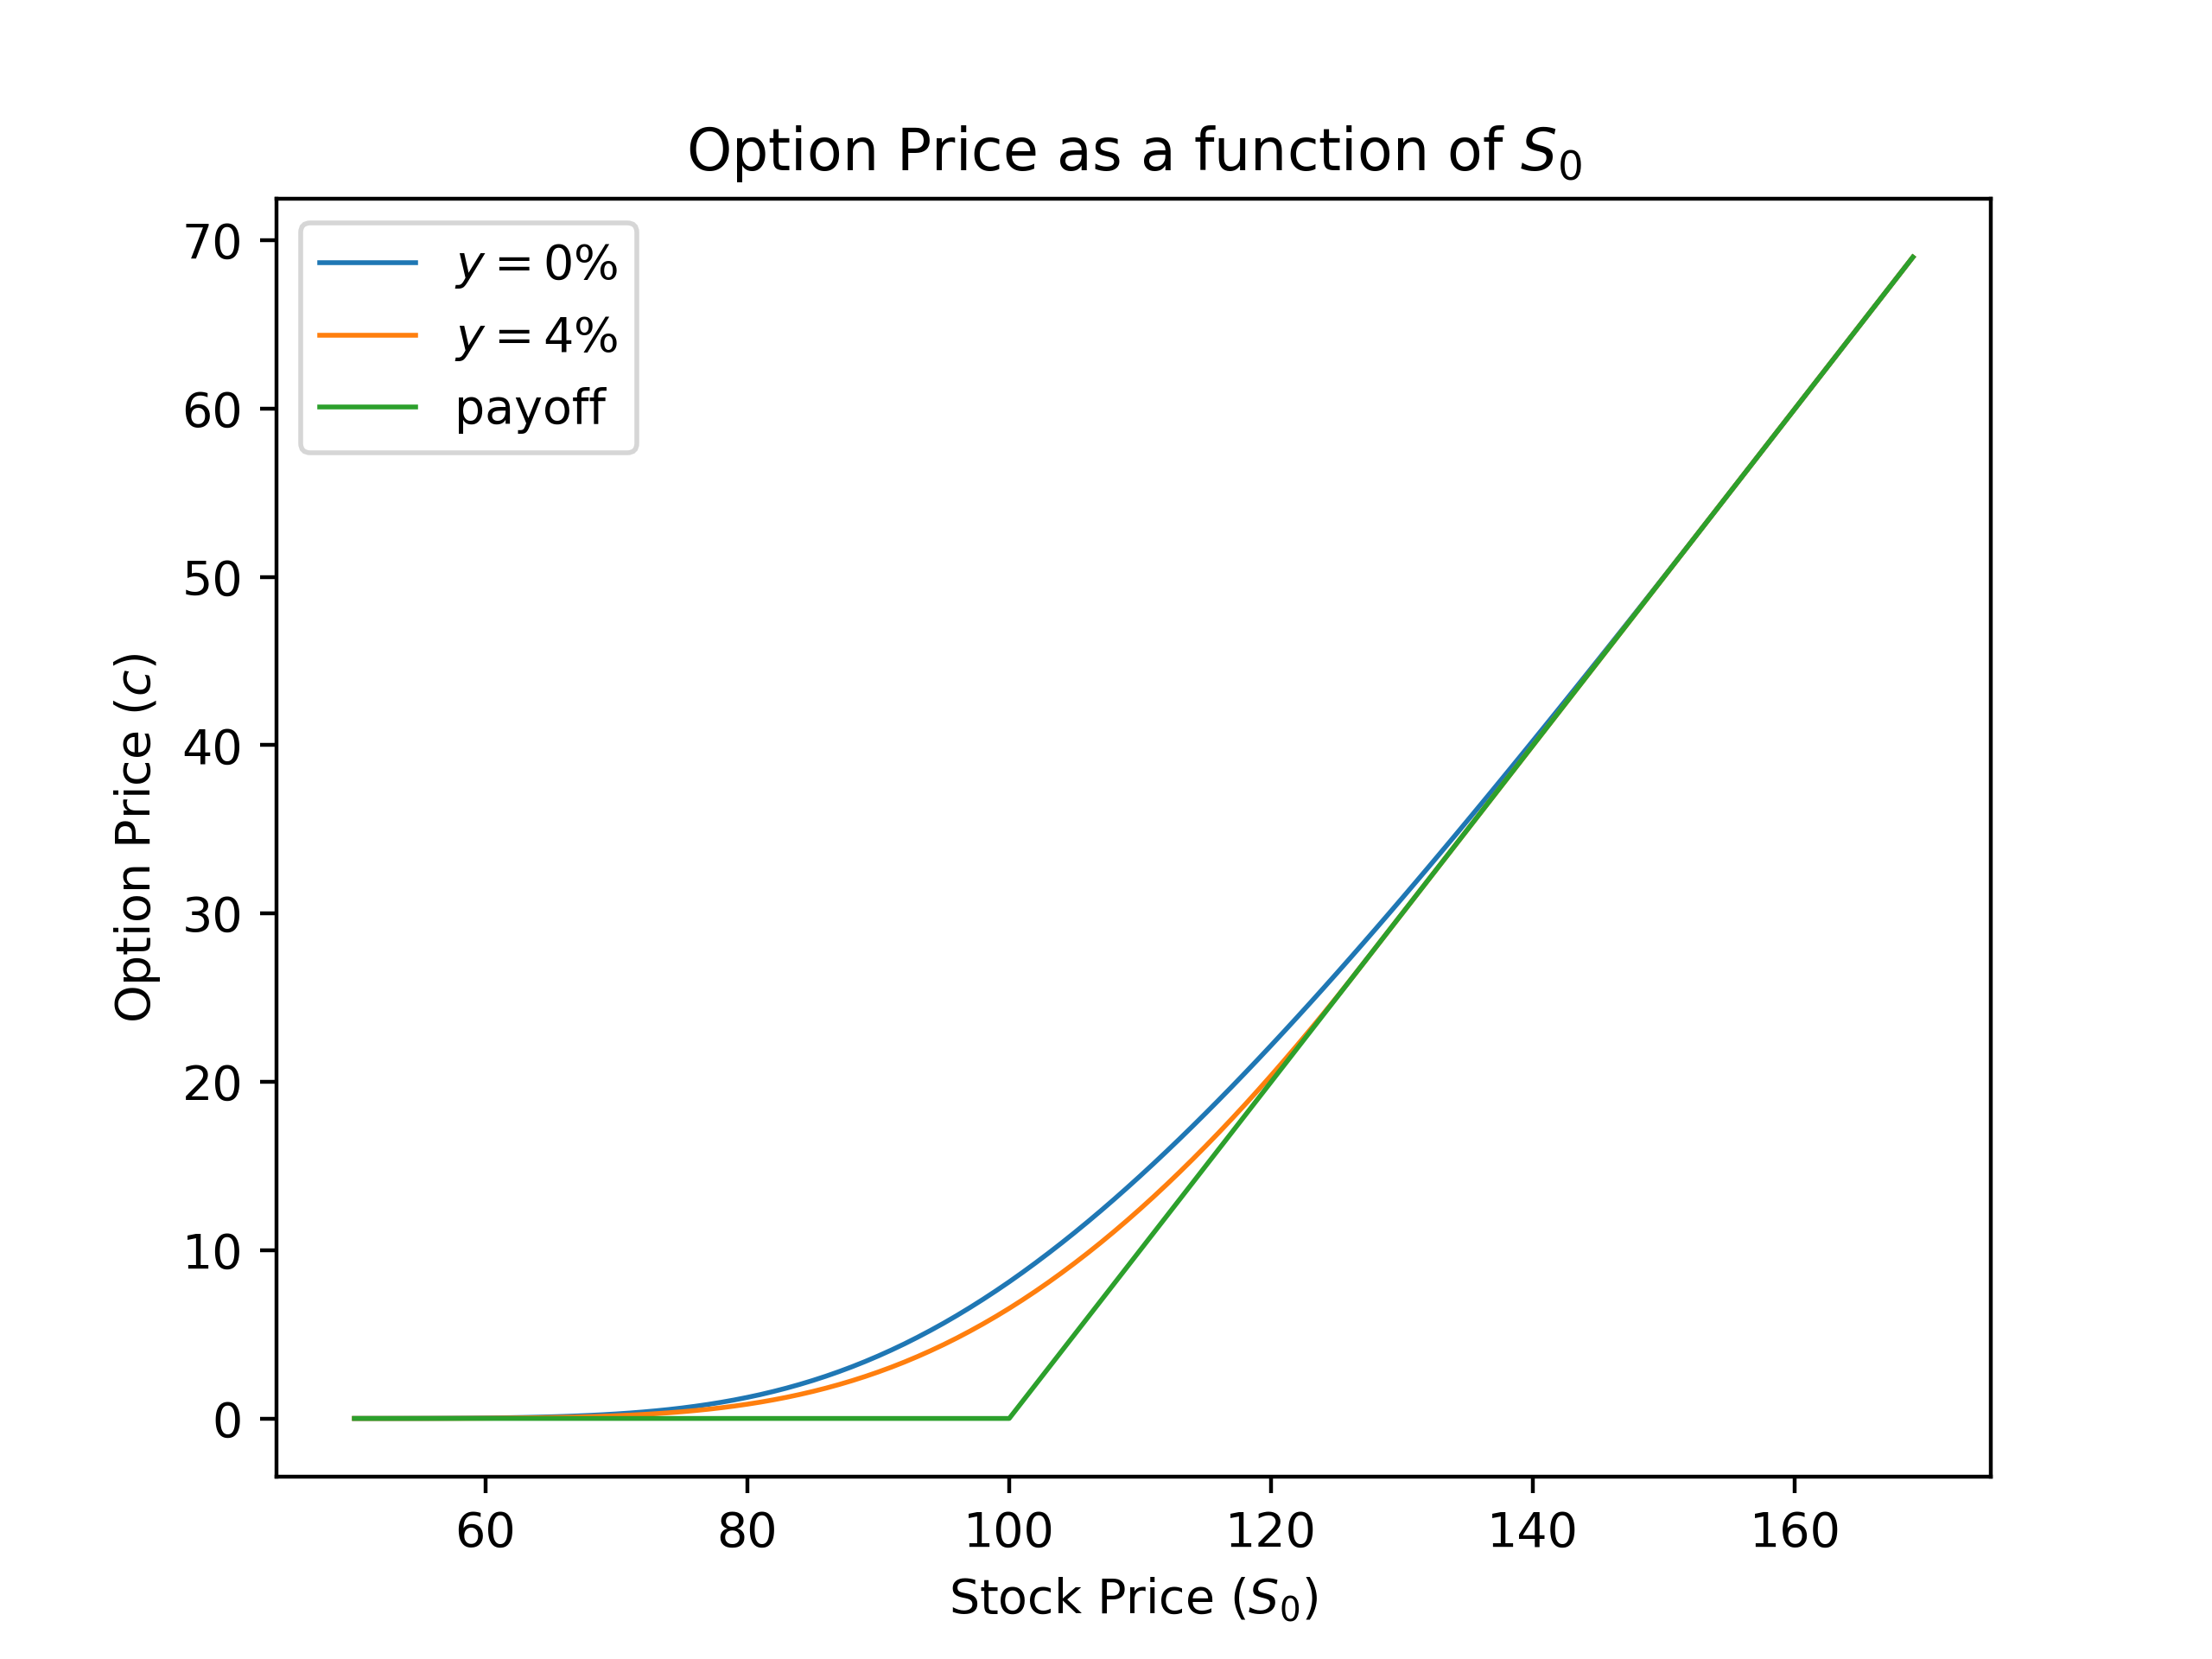
\includegraphics[width=90mm]{images/q4_function_of_S0.png}
	\caption{CRR binomial call price as a function of initial stock price $S_0$}
	\label{q4S0}
\end{figure}

Figure \ref{q4S0} shows that the price of the American call option increases as $S_0$ increases. The contract gives the holder the right to buy the underlying asset at strike price $K=\$100$, and thus the option increases in value as the inital price of the underlying asset $S_0$ increases. For high values of $S_0$, the option price converges towards the intrinsic value of the underlying option as the ability to exercise early comes into play.

When increasing the dividend yield (from $4\%$ to $8\%$), the value of the option decreases. This is due to the fact that the value of the underlying option decreases with the dividend amount after the dividend date. When this occurs, the ability to buy the asset at the strike price is less valuable, and thus the option is priced lower. As for the put option in Question 3, the price difference goes towards zero for values of $S_0$ that enables early exercise (high values of $S_0$ in this case).

\begin{figure}[H]
	\centering
	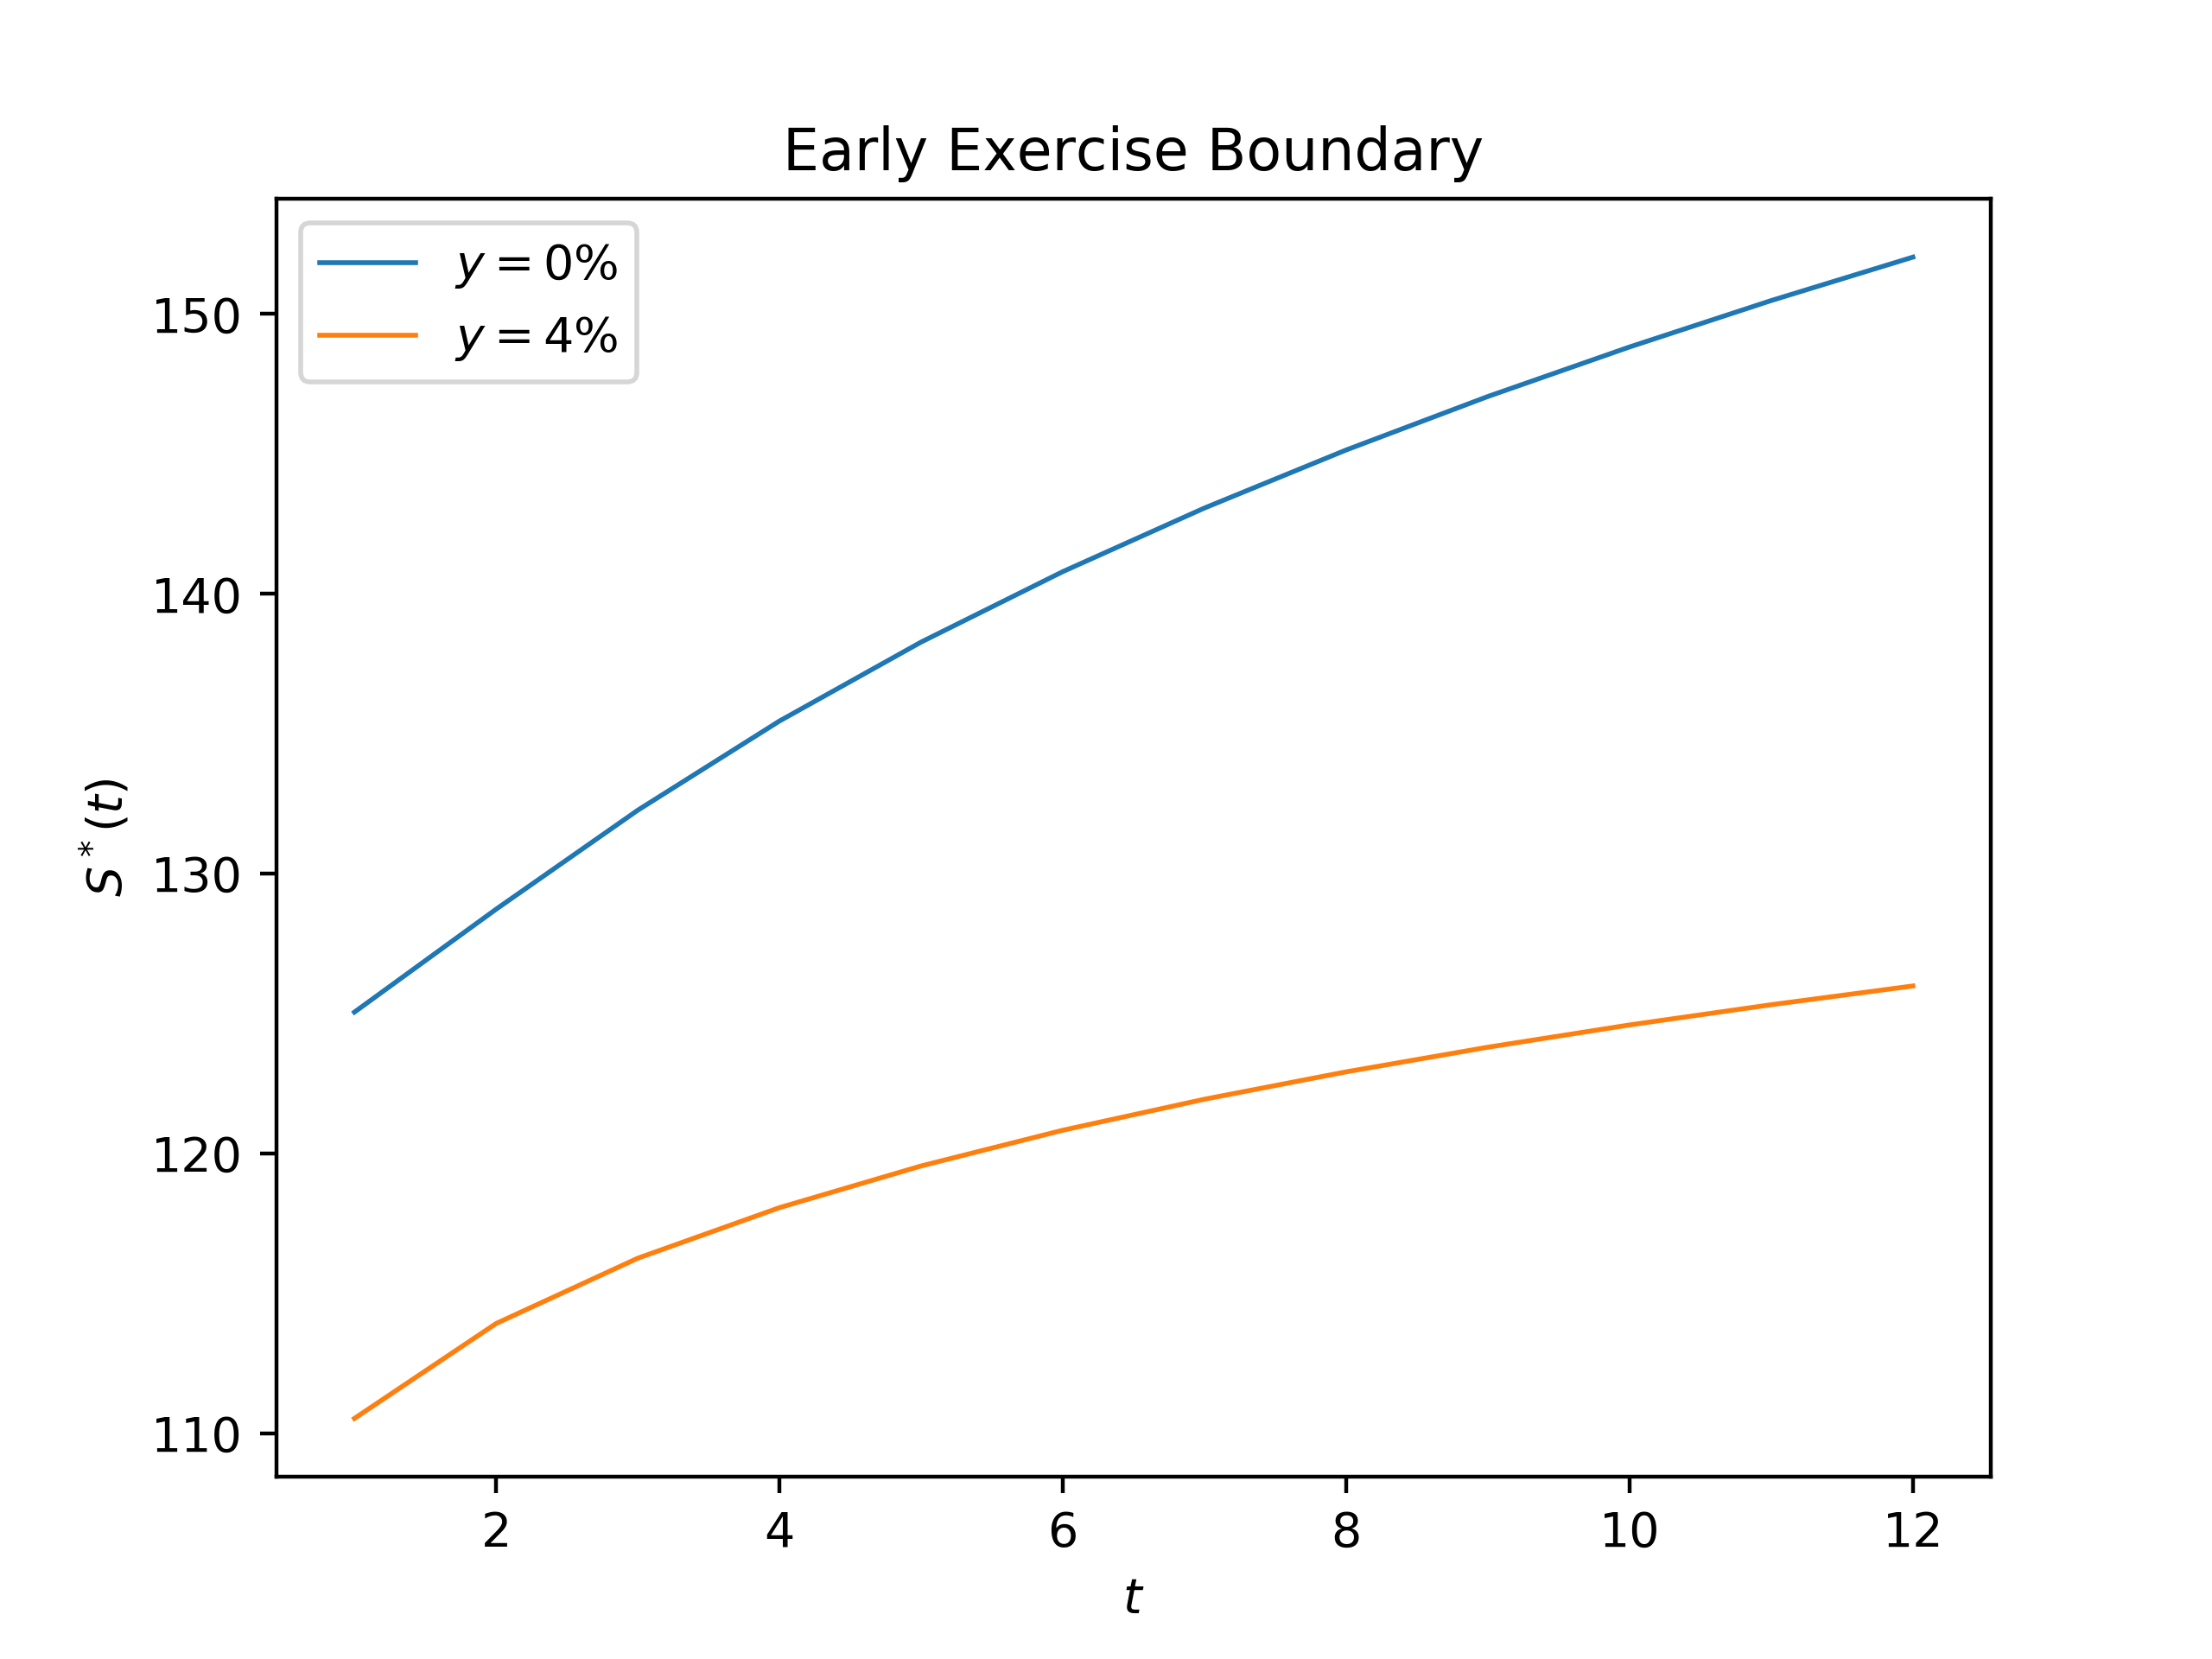
\includegraphics[width=90mm]{images/q4_critical.png}
	\caption{The critical price $S^*(t)$ as a function of time to maturity $t$ ranging from 1 month to 1 year.}
	\label{q4Crit}
\end{figure}


\begin{table}[H]
	\begin{center}
		\begin{tabular}{ || c | c | c ||}
		\hline
		T & $S^*$ ($q=4\%$) & $S^*$ ($q=8\%$)\\ 
		\hline
		1 & 125.0543  & 110.536\\ 
		2 & 128.7319  & 113.928\\ 
		3 & 132.2693  & 116.2616\\ 
		4 & 135.4561  & 118.0681\\ 
		5 & 138.2776  & 119.5583\\ 
		6 & 140.7946  & 120.8348\\ 
		7 & 143.0679  & 121.9429\\ 
		8 & 145.1413  & 122.9212\\ 
		9 & 147.0523  & 123.8013\\ 
		10 & 148.8218 & 124.5968\\ 
		11 & 150.4804 & 125.3194\\ 
		12 & 152.032  & 125.9898\\ 
		\hline 
		\end{tabular}
	\end{center}
	\caption{asdasd}
	\label{q4table}
\end{table}


For time to maturity ranging from 1 to 12 months, the critical price $S^*$ was numerically approximated by calculating the difference between the option price and the intrinsic value of the option for increasing values of $S_0$. This was done with a step size of 1 until an upper bound was found at which the difference exceeded 0.005. The interval was then updated and the step size was divided by 10. The process was repeated until the step size was 0.0001. At this point the approximation of $S^*$, i.e. the lowest value of the stock price that provided a difference less than 0.005, was well within the required tolerance. The results are presented in the plot and table above. (See appendix \ref{critical} for more details)

Figure \ref{q4Crit} and table \ref{q4Crit} show the critical prices for the call option as a function of time to maturity (1-12 months). When increasing the dividend yield to $8\%$, the call option decreases in value for the holder due to the fact that the underlying asset decreases in value (with the dividend amount). This in turn means that the time value of the call option decreases, and as such the early exercise boundary indicating when it is optimal to exercise the option before maturity moves to a lower level in terms of $S_0$. The reason for this is that a lower stock price and therefore return upon exercising the option is required for an early exercise to be optimal. 
	

\pagebreak

\appendix
\section{Code Appendix}
\subsection{CRR Binomial Code}\label{binomial}
\lstinputlisting[language=C++]{../src/CPP/binomial.cpp}

\subsection{Black \& Scholes Code}\label{blackscholes}
\lstinputlisting[language=C++]{../src/CPP/black_scholes.cpp}

\subsection{Options Utils Code}\label{options}
\lstinputlisting[language=C++]{../src/CPP/options.cpp}
\lstinputlisting[language=C++]{../src/CPP/options.h}

\subsection{Critical Price Code}\label{critical}
\lstinputlisting[language=C++]{../src/CPP/critical.cpp}
\lstinputlisting[language=C++]{../src/CPP/critical.h}

\subsection{Main Code}\label{main}
\lstinputlisting[language=C++]{../src/CPP/main.cpp}

\end{document}
